\documentclass[a4paper]{report}
\usepackage{unifrrr}
\usepackage{graphicx}
\usepackage[latin1]{inputenc}
\usepackage{float}
\usepackage[colorlinks=false, pdfborder={0 0 0}]{hyperref}
\usepackage{verbatim}
\usepackage{hyperref}
\usepackage{cite}
\usepackage{bibgerm}
\usepackage[english]{babel}
\usepackage{listings}
\usepackage{color}
\usepackage{appendix}
\usepackage{minitoc}
\usepackage[onehalfspacing]{setspace}
\usepackage[nottoc]{tocbibind}
\usepackage{multirow}
\usepackage{longtable}
\definecolor{javared}{rgb}{0.6,0,0} % for strings
\definecolor{javagreen}{rgb}{0.25,0.5,0.35} % comments
\definecolor{javapurple}{rgb}{0.5,0,0.35} % keywords
\definecolor{javadocblue}{rgb}{0.25,0.35,0.75} % javadoc


\lstset{language=Java,
basicstyle=\ttfamily\footnotesize,
keywordstyle=\color{javapurple}\bfseries,
stringstyle=\color{javared},
commentstyle=\color{javagreen},
morecomment=[s][\color{javadocblue}]{/**}{*/},
numbers=left,
numberstyle=\tiny\color{black},
stepnumber=1,
numbersep=10pt,
tabsize=4,
showspaces=false,
showstringspaces=false,
captionpos=b}

\begingroup
    \catcode `\@ = 11
    \catcode `\~ = 13
    \catcode `\% = 12
    \protected\long\gdef\cmt@remove#1%~{\endgroup}
    \ifdefined~
        \global\let\cmt@old~
    \else
        \global\let\cmt@old\relax
    \fi
    \protected\gdef~{\begingroup\catcode`%=12
        \futurelet\next\cmt@}
    \protected\gdef\cmt@
      {\ifx%\next
           \expandafter\cmt@remove
       \else
           \endgroup\expandafter\cmt@old
       \fi}
\endgroup


\setcounter{secnumdepth}{3}
\setcounter{tocdepth}{3}

%--------------------------------------------------------------------


%The body of the LaTeX file
\begin{document}  



%Including of the title page. See titlepage.tex file
%Starting the title page. A \begin command always ends with a \end command
\begin{titlepage} 
	%Center all the following stuff
	\begin{center}
		
		%Include the unifr.jpg file from ./images. \\ is a line break
		
\includegraphics[scale=2]{images/unifr.jpg}\\
		
		%Do a vertical space of 0.5 cm
		\vspace{0.5cm}
		
		
	
		\vspace{2cm}
		
		\begin{Large}
		Master Thesis\\
		\end{Large}
		
		\vspace{2cm}
		
		%Start a huge font
		\begin{huge}
			%Sans serif
			{\sf \bf Crowdsourced Product Descriptions and Price Estimations}
		\end{huge}
		
				
		\vspace{2cm}
		
		 Steve Aschwanden\\
		 Dammstrasse 4\\
		 CH-2540 Grenchen\\
		 steve.aschwanden@students.unibe.ch\\
		 05-480-686\\
		
		\vspace{1.5cm}
		
		{\bf Supervisor}\\
		Dr. Gianluca Demartini\\
		C302, Bd de P�rolles 90\\
		CH-1700 Fribourg\\
		demartini@exascale.info\\
		\vspace{2.5cm}
		
		
		Grenchen, \today\\
		
				
	\end{center}
\end{titlepage}


\pagenumbering{arabic}
\pagestyle{plain}
\newpage

\chapter*{Declaration}
\thispagestyle{empty}

\vspace{0.2in}
I declare that this written submission represents my ideas in my own words and where others' ideas or words have been included, I have adequately cited and referenced the original sources. I also declare that I have adhered to all the principles of academic honesty and integrity and have not misrepresented or fabricated or falsified any \mbox{idea/data/fact/source} in my submission. I understand that any violation of the above will be cause for disciplinary action by the Institute and can also evoke penal action from the sources which have thus not been properly cited or from whom proper permission has not been taken when needed.
\vspace{1in}
%\begin{table*}[hb]
\begin{center}
\begin{tabular*}{\textwidth}{@{\extracolsep{\fill}} lr }
\vspace{0.5in}
& Steve Aschwanden, 05-480-686\\
Grenchen; \today: & \hrulefill \\
& (Signature)\\
\end{tabular*}
\end{center}
\chapter*{Acknowledgements}
\thispagestyle{empty}
I like to acknowledge ...
\clearpage
\chapter*{Abstract}
\thispagestyle{empty}
The creation of auctions for the online marketplace eBay is time consuming and repetitive. The first step for selling an item is taking pictures of it. To complete the auction, the user has to provide a title, description, category and other predefined parameters. One of the most important step is the definition of a starting price.\\\\
Crowdsourcing is used to generate the required information for a complete auction based on several images. The complex task is split into multiple subtasks. The thesis presents a pure and a hybrid crowdsourcing approach. Different experiments were made to investigate the behaviour of the crowd.\\\\
A promised commission for successful auctions has the biggest influence to the quality of the workers. A majority favours the results of this experiment over the descriptions of the corresponding real online auction. The workers did the most accurate price predictions if the actual market price of the items is provided.\\\\  
The results of the executed experiments show the potential of the crowd. If all the strength of the single variations will be combined and the task design is improved slightly then the generated contents can be used to create real auctions on eBay in the future.
\clearpage


\dominitoc
\tableofcontents
\newpage

\listoffigures

\listoftables

\lstlistoflistings

\chapter{Introduction}
eBay Inc.\footnote{http://www.ebay.com} is one of the world's largest online marketplaces and reported 128 million active users worldwide during the last quarter of the year 2013. Online auction platforms make consumer-to-consumer transactions possible. The seller can present articles by uploading pictures and describing them. The creation of an auction is time consuming and needs a lot of investigations. Searching for descriptions on the internet or finding a selling price for the same or similar article, for example. In 2005, Jeff Howe and Mark Robinson created a term called 'Crowdsourcing' which is a combination of the words crowd and outsourcing. The idea behind the term is to outsource different tasks, which are difficult to solve by machines, to the crowd. To reduce the costs of collecting information for an article to sell on an auction platform, tasks will be created and outsourced to the crowd. Amazon Mechanical Turk\footnote{http://www.mturk.com}, short MTurk, is a crowdsourcing marketplace which enables requesters to publish human intelligence tasks (HITs). The workers can solve these tasks and earn money for good work.

\section{Statement of the problem}
The first step of creating an online auction is mostly to take pictures of the corresponding item. This help the buyers to get information about the state and quality of the article. After that the item needs a short and clear description, some properties (category, state) and a starting offer. If the seller wants to create a lot of different auctions, the whole procedure is time consuming and boring. A price estimation of an article can be difficult, because the background knowledge is missing and other auctions to compare aren't available at any time. Machines aren't able to solve all these steps by them self, because the spectrum of the articles is huge and image processing methods aren't capable to classify them all correctly. To get all the needed parts of an online auction, a human powered approach is necessary. Crowdsourcing platforms provide the possibility to solve tasks, which are difficult to handle for a computer.

\section{Existing research}
Some similar existing research projects are illustrated in this section: 
\subsection{Crowdsourcing}
The idea of the thesis is similar to a project called ''PlatMate''\cite{platemate} where workers analyse the content of food photographs. The processing pipeline consists of three major steps and put out the calorie values of every ingredient on the picture. All steps were performed by workers of a crowdsourcing platform. The accuracy of the calorie estimations of the system is almost as good as estimations from different trained experts. 
\subsection{Price Estimation}
The idea of predicting the end price of online auctions is not new. People from the Accenture Technology Labs\footnote{http://www.accenture.com} tried to do this in 2005 and published some surprising results\cite{ghani}. They collected 1'700 auctions of a specific item during a two-month period to form a training and test set. The end prices of the ground truth are additionally converted to a price class (10\% of the average price) to perform classification algorithms. The accuracy of the classifiers are higher then 70\%.

\section{Goals and objectives}
The thesis has the following goals and their corresponding objectives:
\begin{itemize}
	\item \textbf{Collect auction item properties by the crowd}
	\begin{itemize}
		\item Analyse the composition of an auction item on eBay and select the parts which can be crowdsourced
		\item Form a ground truth including different auctions created by real online auction platform users by using the eBay API
		\item Study literature which covers similar crowdsourcing problems
		\item Design and publish tasks on Amazon Mechanical Turk to gather data from the crowd
		\item Evaluate the quality of the generated content
	\end{itemize}
	\item \textbf{Vary the design of the tasks and investigate the behaviour of the workers}
	\begin{itemize}
		\item Find parameters for the HITs
		\item Analyse the influence on the performance of the workers
	\end{itemize}
	\item \textbf{Try to improve the initial solution by implementing a hybrid approach}
	\begin{itemize}
		\item Search for image processing or machine learning methods which can simplify and/or support a human intelligence task
		\item Implement the methods and adapt the design of the tasks
		\item Publish the new tasks on the same crowdsourcing platform
		\item Evaluate the results and compare them to the first solution 
	\end{itemize}
\end{itemize}

If the main goals of the thesis are fulfilled, some \textit{optional} goals can be covered by the thesis:
\begin{itemize}
	\item \textbf{Implement a web application which combines the created subtasks to a complete workflow}
	\begin{itemize}
		\item Find a web application framework which provide an API in the same programming language as the Amazon Mechanical Turk API
		\item Create a workflow which put all the subtasks together to an overall solution
		\item The user can manage the items (upload pictures to create new items, edit and remove items) and directly create an online auction
	\end{itemize}
\end{itemize}

\section{Organisation}
The thesis report is organised in multiple chapters. At the beginning of the document, the eBay marketplace and the corresponding API will be investigated (Chapter \ref{chap:ebay}). Then the theoretical background knowledge about crowdsourcing is summarised (Chapter \ref{chap:crowdsourcing}). The learned theory was used to build up a workflow to generate online auction contents (Chapter \ref{chap:implementation}). The observations of the executed experiments are concluded in the next chapter (Chapter \ref{chap:evaluation}). Some ideas for improvements and a short discussion of the pros and cons of the implemented approach are part of the last chapter (Chapter \ref{chap:conclusion}). All the ground truth items, some plots and tables which didn't find a place in the report are listed in the appendix section.

\chapter{eBay Online Marketplace}
\label{chap:ebay}
\section{History}
eBay was founded 1995 in San Jose (CA) as AuctionWeb by Pierre Omidyar. One year later, eBay bought a third-party licence from Electronic Travel Auction to sell plane tickets and other travelling stuff. During the year 1996, over 200'000 auctions were available on the website. At the beginning of 1997 the number of auctions exploded (about 2 million articles). In the same year the company get their well-known name eBay and received 6.7 million dollar from the venture capital firm Benchmark Capital. The company went public on the stock exchange on September 21, 1998 and the share price increased from 18 to 53.5 dollar on the first day of trading. Four years later the growth continues and eBay bought the online money transfer service PayPal. eBay expanded worldwide in early 2008, had hundred millions of registered users and 15'000 employees. Today, the firm is one of the world's largest online marketplaces. During the fourth quarter of the year 2013 about 128 million active users were reported. A cell phone was sold every 4 seconds, a pair of shoes every 2 seconds and a Ford Mustang every 55 minutes.

\section{Auction item composition}
Every eBay user has the possibility to create auctions for different kind of items. To present the article, the seller has to provide accurate information about it. The standard eBay auction consists of the following fields:
\begin{itemize}
	\item \textbf{Title} The title of the item is limited to 80 characters. The sellers should use descriptive keywords to clearly and accurately convey what they are selling
	\item \textbf{Description} The description is the opportunity to provide the buyers with more information about the item
	\item \textbf{Category} An item can have multiple predefined categories. eBay provides a list of categories which the seller can select
	\item \textbf{Condition} The condition of the item is dependent on the selected category. eBay provides different condition schemas. For clothing items the seller can select between 'New with tags', 'New without tags', 'New with defects' or 'Pre-owned'. For other categories like books, other condition values are present: 'Brand new', 'Like new', 'Very good', 'Good', 'Acceptable'
	\item \textbf{Pictures} To visualise the item the auction creator can upload up to twelve pictures. The first image is important, because it appears next to the item's title in the search result. The pictures will be stored for 90 days on the eBay servers.
	\item \textbf{Shipping costs} The seller has to tell the future buyers how much shipping will cost. There are three possibilities:
	\begin{itemize}
		\item Free shipping
		\item Flat shipping, same cost to all buyers
		\item Shipping rate tables, eBay calculates the cost for every individual buyer dependent on the location
	\end{itemize}
	\item \textbf{Duration} An auction can have a duration of 1, 3, 5, 7 or 10 days. If the item has a fixed price, the auction is finished if a buyer is willing to pay this price.
	\item \textbf{Pricing} The seller can select a starting price and then the bidding will start at this price. A 'But it now' option is also available. The buyer can skip the bidding process.
	\item \textbf{Payment} The seller has to select the desired paying method like 'PayPal' or 'Payment upon pickup'
\end{itemize}

\section{APIs}
eBay provides multiple APIs for developing third party applications. This allows developers to search for auctions or create listings over the XML format. Three main interfaces are available:
\begin{figure}[h!]
\centering
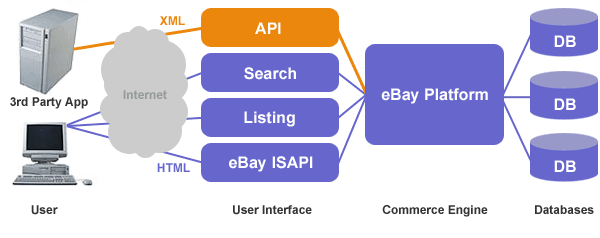
\includegraphics[scale=0.5]{images/api-flow.png}
\caption{eBay API overview}
\label{ebayAPI}
\end{figure}

\subsection{Trading API}
Developers use the Trading API to build applications such as selling and post-sales management applications, manage user information, and initiate the item purchase flow on eBay. The API is available in .NET, Java, PHP and Python.

\subsection{Shopping API}
The Shopping API provides a search engine for user information, popular items and reviews. The API is available in PHP and Python. Example calls for this API are:
\begin{itemize}
	\item \textit{findProducts()}: Search for products by keywords or ProductId
	\item \textit{GetSingleItem()}: Buyer specific view of an item
	\item \textit{GetUserProfile()}: Get the user profile and feedback information
\end{itemize}

\subsection{Finding API}
The Finding API provides access to the next generation search capabilities on the eBay platform. The developer can search and browse for items based on keyword queries, categories or an image. The API is available in .NET, Java and Python. Example calls for this API are:
\begin{itemize}
	\item \textit{findCompletedItems()}: Find the items which are listened as completed or no longer available on eBay
	\item \textit{findItemsByCategory()}: Find items in a specific category
	\item \textit{findItemsByImage()}: Find items which have a high similarity to a given image
\end{itemize}

\subsection{Example}
The following listing in Python illustrate the functionality of the Finding API. The developer has to register to the eBay developers program first. After that, a application ID can be created. This is necessary to get access to the eBay databases. A functioning Python environment and the additional eBay Python SDK are requirements to successfully execute the example
\lstset{language=Python,caption={eBay Finding API example},label=findingapi_example}
\begin{lstlisting}
from ebaysdk.finding import Connection as Finding
from ebaysdk.exception import ConnectionError
import json

try:
    api = Finding(appid='Universi-3c25-4b4e-b3e6-8c2568808b12')
    api.execute('findCompletedItems', {
        'keywords': 'ford mustang',
        'itemFilter': [
            {'name': 'ListingType',
             'value': 'Auction'},
            {'name': 'Currency',
             'value': 'USD'},                
            {'name': 'SoldItemsOnly',
             'value': 'true'},                 
        ],        
        'sortOrder': 'StartTimeNewest',
        })
    response = json.loads(api.response_json())
    
    print response['searchResult']['item'][0]
    
except ConnectionError as e:
    raise e  
\end{lstlisting}
The initialisation of the application is done on line 6. A correct application ID is required. Then the API call \textit{findCompletedItems()} is executed with some keywords and filter options. Only the newest auctions with at least one bidder and a payment in US dollar will be returned. The function \textit{response\_json()} (on line 19) returns the first 100 items by default. At the end, the first result will be printed to the console. Here is a shorter simplified version with the most important fields of the output:
\begin{table}[h!]
	\begin{center}
	\begin{tabular}{| l | l |}
		\hline
		\textbf{Name} & \textbf{Value} \\
		\hline
		itemId & 281273507096 \\
		\hline
		title & 2014 Hot Wheels Super Treasure Hunt 71 Mustang Mach 1 \\
		\hline
		categoryName & Diecast-Modern Manufacture \\
		\hline
		shippingType & Calculated \\
		\hline
		currentPrice & 18.5 USD \\
		\hline
		bidCount & 1 \\
		\hline
		paymentMethod & PayPal \\
		\hline
		conditionDisplayName & New \\
		\hline
		startTime & 2014-02-25T04:32:17.000Z \\
		\hline
		endTime & 2014-02-25T05:27:14.000Z \\
		\hline
	\end{tabular}
	\end{center}
	\caption{eBay Finding API example output}
\end{table}


\chapter{Crowdsourcing}
\label{chap:crowdsourcing}
\section{Introduction}
In 2005, Jeff Howe and Mark Robinson created the term `Crowdsourcing' after a discussion about how businesses can outsource their work to individuals over the internet. There exist multiple definitions in the literature. Enrique Estell\'{e}s-Arolas and Fernando Gonz\'{a}lez Ladr\'{o}n-de-Guevara analysed over 40 definitions of crowdsourcing and developed a new integrating definition \cite{estelles}:\\\\
``Crowdsourcing is a type of participative online activity in which an individual, an institution, a non-profit organization, or company proposes to a group of individuals of varying knowledge, heterogeneity, and number, via a flexible open call, the voluntary undertaking of a task. The undertaking of the task, of variable complexity and modularity, and in which the crowd should participate bringing their work, money, knowledge and/or experience, always entails mutual benefit. The user will receive the satisfaction of a given type of need, be it economic, social recognition, self-esteem, or the development of individual skills, while the crowdsourcer will obtain and utilize to their advantage that what the user has brought to the venture, whose form will depend on the type of activity undertaken.''
\section{Platforms}
\subsection{Amazon Mechanical Turk}
The project was introduced in 2005 and is part of the Amazon Web Services\footnote{http://aws.amazon.com}. Requesters can post tasks known as HITs (Human Intelligence Tasks) which can be solved by workers (Amazon uses another term: Turkers). MTurk provides a web-based user interface and a couple of APIs in different programming languages (.NET, Java, Python, PHP, Perl, Ruby) to manage tasks. The first action of the requester is to create a HIT consisting of mandatory fields: 
\begin{itemize}
	\item \textbf{Title} The requester must describe the idea of the HIT in at most 128 characters. 
	\item \textbf{Description} A more detailed description of the task which cannot be longer than 2'000 characters. 
	\item \textbf{Question} Every task has to contain questions to collect information from the crowd. The requester can decide between three question data structures. 
	\begin{itemize}
		\item \textit{QuestionForm} The simplest form to create questions in a HIT. MTurk uses a special XML language to define tasks which has some restrictions. For example, JavaScript and CSS are not allowed. 
		\item \textit{ExternalQuestion} MTurk will display a requester defined external webpage and the answers to the questions will be collected on the external website and send back to MTurk. This question data structure is used to overcome some restrictions of the platform like using JavaScript or to display CSS defined content. 
		\item \textit{HTMLQuestion} This structure is a mixture between QuestionForm and ExternalQuestion. The requester has not to host an external website to provide a HTML based form. 
	\end{itemize}
	\item \textbf{Reward} If the workers will successfully completing the HIT, then they will receive a predefined amount of money from the requester. 
	\item \textbf{Assignment duration in seconds} The time in which the workers have to complete the task after they have accepted it. The time has to be between 30 seconds and one year. 
	\item \textbf{Lifetime in seconds} The lifetime of a HIT defines the amount of time a task is acceptable for the workers. After the time elapsed, the HIT will no longer appear in the search results.
\end{itemize}
and some important, optional fields: 
\begin{itemize}
	\item \textbf{Keywords} Comma separated keywords which describe the task (max. 2'000 characters). 
	\item \textbf{Max assignments} Number of times a HIT can be completed. The default values is one. 
	\item \textbf{Qualification requirement} Requesters can define requirements to process a task for the workers. For example, only workers who have more than 100 approved assignments can start working on a requesters HIT. 
\end{itemize}
After the tasks are designed, the requesters have to test them on the Amazon Mechanical Turk Developer Sandbox platform which is a simulated environment. If the requester is happy with the appearance of the HIT, the task can be published on the productive MTurk platform. Turkers have now the possibility to accept the HITs and complete the assignments until the lifetime is expired. After the HIT is completed, the requesters can take a look at the results and have to decide if they want to accept or reject the work. The workers will receive the predefined amount of money only for an accepted task. 

\subsection{Crowdflower}
A platform for large-scale data projects was founded in 2007. Crowdflower\footnote{http://www.crowdflower.com} has over 50 labor channel partners, Amazon Mechanical Turk for example, where the created tasks are published. The partner websites or communities are responsible to manage the registration and payment of their workers. The company offers enterprise solutions and enables a higher degree of quality control. `Gold standard data' (cf. \ref{sub:honeypots}, page \pageref{sub:honeypots}) and `Peer review' are two provided quality control techniques. `Peer review' gives the requesters the chance to improve the data by a second pass. A workflow management tool helps to link different jobs together. At the time of writing these lines, over one billion tasks are completed by workers domiciled in 208 different countries. Big companies like eBay use the Crowdflower service for their projects \cite{crowdflower_casestudy}. Over the past years, the company has completed over 15 projects. The improvement of the product categorisation algorithm was one of them.
\section{Patterns}
This section presents two probed ways to get useful information from the crowd.
\subsection{Find-Fix-Verify}
The Find-Fix-Verify pattern was introduced by the Soylent paper \cite{soylent}. The pattern divides the overall task into three stages. During the Find stage, the workers will identify patches of work done by the crowd or create new patches. For example, the workers have to select a sentence which seems to be incorrect and will need further investigations during the Fix phase. Some workers will revise the identified patches and try to provide alternatives. The last step of the pattern will present the generated alternatives during the Fix stage to a few new workers in a randomized order. The answer with the most votes (plurality voting) will be used to replace the identified patch during the first phase. The creators of the new suggestions will be suspended so that they cannot vote for their own input.

To illustrate the meaning of the Find-Fix-Verify pattern, the implementation of Soylent will be discussed (Figure \ref{fixfindverify}). The approach begins by splitting a text into paragraphs. During the Find stage, the workers have to identify candidate areas for shortening in each paragraph. If a certain number of workers have selected the same area, then this patch goes to the next stage. Every worker in the Fix stage has to present a shorter version of the identified patch if possible. They also have the possibility to say that the text cannot be reduced. During the last step, the crowd has to select rewrites which have spelling, style, or grammar problems or change the meaning of the sentence significantly. At the end, they remove these patches by a majority voting.
\begin{figure}[h!]
\centering
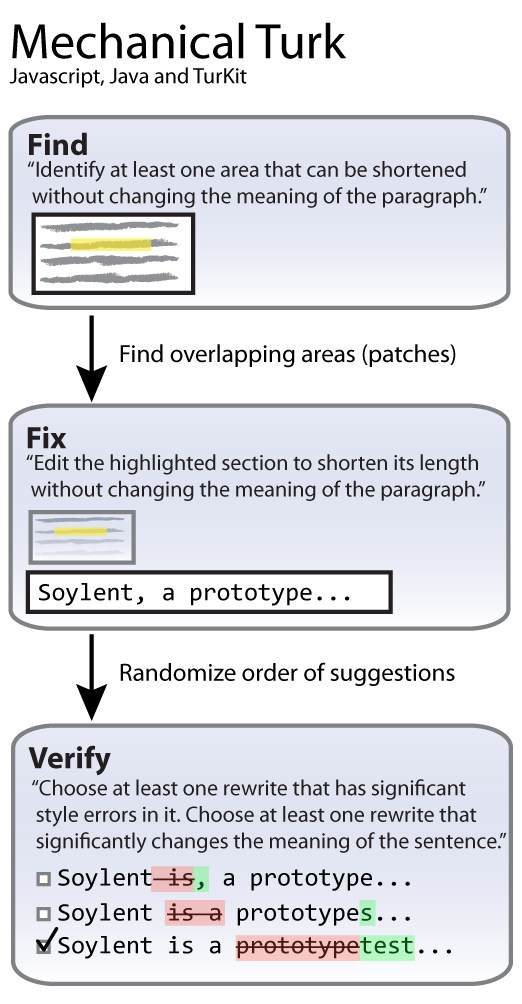
\includegraphics[scale=0.35]{images/soylent_system_overview.png}
\caption{Soylent Fix-Find-Verify pattern}
\label{fixfindverify}
\end{figure}

\subsection{Iterative}
\label{iterative}
Most of the published assignments on MTurk are independent, parallel tasks. However, also iterative sequential tasks can be useful. The authors of the TurKit paper \cite{turkit} implemented a tool which make iterative tasks possible. They developed an example application for creating an image description (Figure \ref{turkit}). During the first iteration, the worker will contribute the initial description of the provided image. The next iteration will show the initial description and a request to improve it. A few workers will evaluate the extension of the description by voting. If the extended description does not receive enough votes, then the iteration will be ignored. The final description is generated after a fixed number of iterations. To make the iterative solution possible, the crash-an-rerun programming model was introduced by the authors of the paper. This model allows a script to be re-executed after a crash without generating costly side-effects. This means, if there is a crash during the second iteration of an iterative problem, the first iteration will be skipped after re-running the script. TurKit is able to persist the state of the program and will never repeat successfully completed tasks. This is helpful for prototyping algorithms.
\begin{figure}
\centering
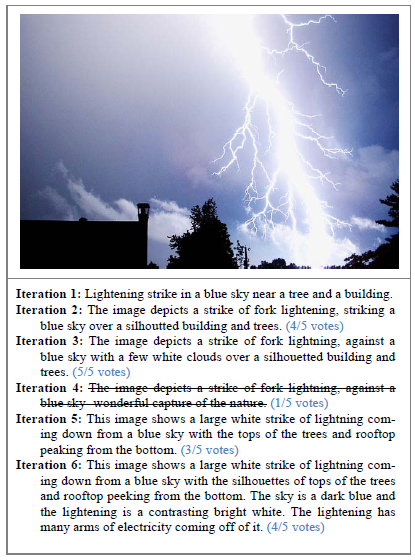
\includegraphics[scale=0.65]{images/turkit_description_example.png}
\caption{Iterative image description created by TurKit}
\label{turkit}
\end{figure}

\section{Design}
If requesters want to create new HITs, then they have to consider some design guidelines\cite{crowdsourcing_tutorial,mturk_bestpractices}: 
\begin{itemize}
\item \textbf{Be as specific as possible in the instructions} If the requesters ask the workers ``Is a Ford Mustang a sports car?'', then this is not the same as they ask them ``Can a Ford Mustang accelerate from 0 to 100 km/h in 3 seconds or less?'' because the second one is clearer and more precise. Sometimes it is useful to hire a technical writer for phrasing task instructions. 
\item \textbf{Instructions have to be easy to read} Instructions should be split into multiple subtasks and presented as a bulleted list. 
\item \textbf{Provide examples} The best way to present the idea of a task is to show one or multiple examples. For example, this can help to avoid uncertainties if the instructions are misinterpreted or the workers have wrong expectations. 
\item \textbf{Mention what will not be accepted} If a worker has to write a paragraph about an encyclopaedia article, the requester can allude in the instructions that copying contents from other website are prohibited.
\item \textbf{Tell the workers which tools they should use.} 
\item \textbf{Give the workers the possibility to write down a feedback about the task} This is important to improve the design of the tasks, or can help to detect spammers. 
\item \textbf{Iterative and incremental development of tasks} The first draft of a task will never be perfect. With the feedbacks and results of the previous iterations, the next one will contain improvements which should avoid foregoing mistakes or design failures.
\end{itemize}

\section{Hybrid}
A lot of information systems use a hybrid crowdsourcing technology. The combination of human intelligence and machine algorithms can lead to powerful information systems which cannot be realised by a pure machine approach. In most cases, the crowd is responsible to verify the created content of machine algorithms or to generate input data for them. 
A closer look at the CrowdSearch \cite{crowdsearch} project helps to illustrate the idea of hybrid systems. The developers implemented an image search system for cell phones. First, the system uses an automated image search to generate a set of candidate pictures. These are packed into multiple identical tasks for validation by humans and published on Amazon Mechanical Turk (Figure \ref{crowdsearch}). A simple majority voting is used to eliminating errors. After the validation of the results, the resulting image will be presented to the user. The drawbacks of such systems are that the hybrid approach generates additional costs for involving humans and the delay between publishing the tasks and receiving the corresponding results. The users of CrowdSearch can define a deadline before they query an image and the system will always return a result after the time is expired, irrespective of whether the crowdsourced tasks are completed or not. 
\begin{figure}
\centering
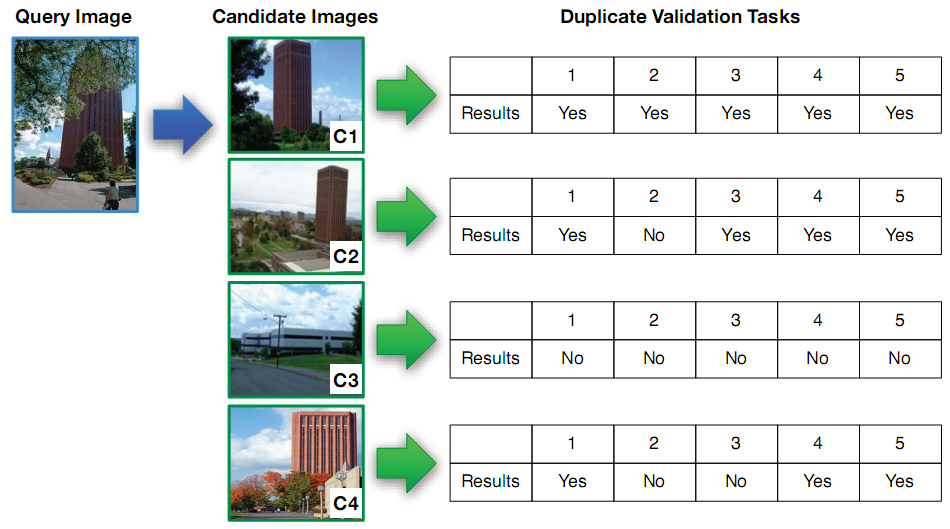
\includegraphics[scale=0.45]{images/crowdsearch_hybrid.png}
\caption{CrowdSearch hybrid image search approach}
\label{crowdsearch}
\end{figure}

\section{Quality Control}
Determination of the quality of completed tasks by the crowd is very important. Workers can be lazy or spammers who want to earn money for free or a minimal amount of work. To evaluate the performance of a single worker, several techniques are available. 
\subsection{Majority Voting}
To reduce the errors of single workers, majority voting can be used. If a majority has the same answer to a question, the requester can assume that the answer is correct. To break ties, an expert is necessary. 
\subsection{Honey Pots}
\label{sub:honeypots}
The requesters include trap questions where they know the correct answer. If the answer of a single worker is incorrect, the requester can exclude the results or reject the task. However, it is not always possible to generate honey pots. 
\subsection{Qualification Test}
MTurk provides the possibility to include a qualification test at the beginning of tasks. The worker has to pass the test to has access to the real tasks and the resulting rewards. The results of the test can be compared to an answer key automatically or by the requesters themselves. The additional effort and the determent of some workers are drawbacks of this procedure.

\section{Workflow}
A workflow is a set of tasks which are interconnected and easier to solve by the crowd. The output of a single subtask will be used for one or multiple subsequent subtasks. The output of the last element of the flow is the result of the entire complex task. There exists a lot of literature which covers the problematic of finding and interconnecting subtasks:\\\\
The process of decomposing complex tasks into simpler ones is not always easy and needs a lot of clarifications. The developers of the Turkomatic\cite{turkomatic} tool had an innovative idea and sourced the workflow decomposition out to the crowd. The workers have to decide how the final workflow should look like and what are the belonging tasks. The system consists of two major parts. The meta-workflow is used to design and execute workflows by applying the price-divide-solve (PDS) procedure. The workers have to recursively divide the complex task into smaller ones until they are simple enough. After this step, the workers will solve the generated tasks and other workers are asked to check the solutions. At the end, the results are combined into a cohesive answer. The second part of the Turkomatic system allows a visualisation of the created workflows and an edit function to manually adapt the crowdsourced results.

Another idea was pursued by the developers of CrowdForge\cite{crowdforge}. They designed a framework to create a workflow by using several partition, map and reduce steps. The partition step splits a larger task into smaller subtasks, the map step lets one or more workers process a specified task. The results of the workers are merged into a single output during the reduce step. The workers should write an encyclopaedia article about a given topic (Figure \ref{crowdforgeflow}), for example. The authors of the paper solved this problem by the presented partition/map/reduce steps. First, the partition step asks the workers to create an outline of the article by defining section headings (e.g. ``History'', ``Geography''). During the map phase, multiple workers are asked to provide a single fact about the section (e.g. ``The Empire State Building celebrated its 75th Anniversary on May 1, 2006'' if it is an encyclopaedia article about ``New York'' and the section heading is ``Attractions''). The workers have to piece the collected facts together to a completed paragraph during the reduction step.

The CrowdForge prototype is written in Python using the Django\footnote{https://www.djangoproject.com} web framework and boto\footnote{https://github.com/boto/boto}, an interface to the Amazon Web Services which is available in Python. The user can define complex flows by creating HIT templates (which can be either a partition, map or reduce task) and dependencies between the templates. Flows are implemented as Python classes. The prototype is also responsible for the sequential coordination between the HITs (including data transfer). Multiple independent flows can be executed simultaneously. One of the limitations is that CrowdForge does not support iteration or recursion. The further development of the project was suspended in 2011.

The same crew developed CrowdWeaver\cite{crowdweaver} which is an advancement of the CrowdForge project. They use CrowdFlower, another crowdsourcing platform, instead of Amazon Mechanical Turk. On CrowdFlower, the requesters can create tasks on multiple markets (including MTurk). Flows can be created visually and does not assume any programming skills. Another feature is the tracking and notification of crowd factors, for example latency or price.
\begin{figure}
\centering
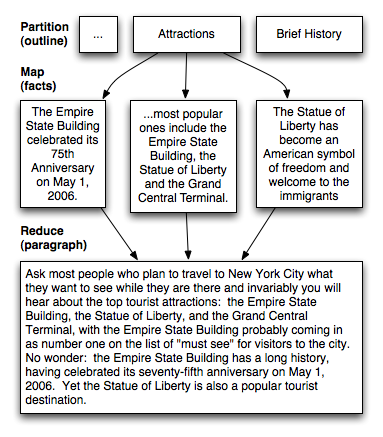
\includegraphics[scale=0.6]{images/crowdforge-article.png}
\caption{CrowdForge example workflow}
\label{crowdforgeflow}
\end{figure}
\section{Incentives}
There are multiple aspects which motivate users to contribute their human power and knowledge. Some of them are described in the following lines.
\subsection{Gamification}
The ESP game\cite{esp} makes the labelling of any kind of images in the web possible. There are no guidelines to provide images and no computer vision method exists which can handle the diversity of all images. Search engines are dependent on accurate image descriptions to represent relevant results. Therefore, another approach was introduced by the article. An online, web-based game was developed to attract workers. Two players are randomly assigned to label the same image simultaneously. There is no possibility to communicate with the game partner. Each player has to guess the description of the image independently without uses the `Taboo words'. These words are evaluated by a prior round and will be ignored for the actual turn. If there is a match between both players, the score will be increased and another image description is detected. The discovered word will only be taken as a valid description and `Taboo word' if a predefined number of players had the same agreement. The duration of the whole game is 150 seconds and both parties can guess as many images as possible within this time. 
During the period of four months, the game was played by 13'630 people and 1'271'451 labels for 293'760 images were generated. These numbers show the power of the idea. The players (crowd) did not know what is going on behind the scenes and they also did not realise the purpose of their inputs.

\subsection{Socialisation}
``Social factors such as the desire to feel a sense of involvement and `belong' to a social group, and the forming and maintaining of interpersonal bounds, are a fundamental human need. Empirical studies also show that social motivation is an important driver for people taking part in online activities, ranging from knowledge contribution to providing emotional support.'' \cite{yu} \\
\\
One example project which use this social incentive is `stackoverflow' \footnote{http://stackoverflow.com/}. People are able to post questions about computer programming issues and other users will provide their help for free. Good answers will receive votes from other contributors and the person who asked the question is authorised to mark an answer as accepted. Hard workers can earn reputation points from other users for questions, answers or edits. A higher reputation score will unlock advanced functionalities. Another way to earn respect from other users is to gather badges. These are achievements which are available in three levels: bronze, silver and gold. ``Answer score of 100 and more'', ``Asked a question with 10'000 views'' or ``Visited the site each day for 30 consecutive days'' are example activities which will be rewarded with badges. The two presented rewards motivate the users of the website to contribute as much content as possible. The community itself is controlling the quality of the answers because experts can remove wrong or low quality statements. Normal users can penalise improper answers by not voting for them. The service sorts answers based on the votes in descending order and the worst evidences will be ignored by the customers.

\subsection{Unintended by-product}
Data from the crowd is collected as an involuntary by-product of the main purpose. One of the most famous projects is reCAPTCHA\cite{recaptcha} which is a further development of the well known Captcha\footnote{http://www.captcha.net/} idea. The method will show distorted characters,  which cannot be recognised by the OCR (Optical Character Recognition) software, to the internet users. The reCAPTCHA acts like a normal Captcha but the inputs will be used additionally to improve text recognition systems.

Another project from the same inventor is Duolingo\footnote{https://www.duolingo.com}. Luis von Ahn has the vision to translate every page in the web into every major language. He hides the main purpose of the service behind a free foreign language learning program. Companies remunerate the founder of the project for translated documents.

\subsection{Financial Reward}
Another possibility to attract workers is the good old money. Crowdsourcing platforms offer to pay them for accepted tasks. If the payment is too low, then workers will not process the tasks. High rewards will attract spammers who deliver bad quality work to collect as much cash as possible in a short amount of time. A research paper from Yahoo \cite{mason} investigates the relationship between financial reward, and the performance of the crowd. They found out, that a higher payment increases the quantity of the work and not it is quality. They proposed to use other incentives like enjoyable tasks or social rewards because the quality of work is the same or better than financial driven approaches. A second advice is that requesters should use as less money as possible only if a payment of the workers is possible. Based on the fact that work will be done faster but not better if a higher gratification will be paid.

Amazon itself does not provide numbers but suggests to take a look at similar HITs to compare rewards \cite{mturk_bestpractices}. A good strategy is also to proof how long it takes to complete the own tasks and then calculate how many tasks can be done in one hour. Different analyses \cite{chilton,ipeirotis} show that the median wage is \$1.38/hour and the average wage \$4.8/hour. The Mechanical Turk Tracker website\footnote{http://mturk-tracker.com} was developed by the author of one of these statistics \cite{ipeirotis} and it is possible to calculate the average cost per HIT for a specific day. On 10th of March 2014, the website tracked 236'370 completed HITs with a total reward of \$23'110 and an average of \$0.097/HIT. These numbers should help the requesters to find an initial price for their tasks. However, there is no general formula to calculate the right costs for an HIT. If the initial price is too low, the workers will ignore those tasks and try to find others with a better revenue/expense ratio. This results in higher completion times. In this case, the requesters should increase the reward. On the other side if the tasks will be completed very fast and the results are not like expected, then a decrease of the reward can be helpful.

\section{Demography}
The workers on the MTurk platform are hidden behind an identification number, no details about gender or country of residence are available. To get detailed information about the workers, researchers from the University of California published surveys in the form of HITs\cite{ross} and presented their results in 2010. They observed the crowd for about 20 months and detected some changes over time. The number of Indian workers raised significantly within one year and approximately one third of the workers were from there. The majority of the turkers was located in the United States (56\%) and every tenth in the United Kingdom, Canada or Philippines. The distribution between female and male participants was nearly equal and most of them were between 18 and 35 years old. A very interesting fact is that 41 percent of the workers were highly educated (Bachelor degree). The authors of the paper also provided numbers about the financial situations of the crowd.  A fifth needed the money to always or sometimes make basic end meets, 30 percent to buy for nice extras. 
Unfortunately, the presented facts are four years old but no current numbers are available for the Amazon Mechanical Turk platform.



\chapter{Implementation}
\label{chap:implementation}
\section{Pure approach}

\subsection{Ground truth}
Real eBay auctions were collected by the API to generate the ground truth for the crowdsourcing experiments. The online auction platform divides their items in eight main categories: Motors, Fashion, Electronics, Collectibles \& Arts, Home \& Garden, Sporting Goods, Toys \& Hobbies and Deals \& Gifts. The ground truth consists of seven items from every category with the exception of the Motor's and Deals \& Gits sections, because the API can't search for items in these categories. First, some keywords were created to touch the desired category: ''Swiss Watch'' (Fashion), ''Smartphone'' (Electronics), ''Football Trading Card'' (Collectibles), ''Coffee Machine'' (Home), ''Soccer shoes'' (Sporting Goods), ''Action Figure'' (Toys) and ''Handbag'' (Fashion). The goal was also to have gender specific and neutral items. An action figure is used by male persons normally, the handbag by females and a smartphone by both. The Finding eBay API provides the method \textit{findCompletedItems} which takes keywords as a parameter and returns a list of completed auction items. The Python script search for the first sold item which uses US dollar as currency, has a description longer than one-hundred characters and contains of at least three images. Only three images were kept, because most of the auctions present the items with a top, front and side view. Another reason is the clarity for the crowdsourcing tasks. Every ground truth entry has the attributes title, description, category, condition, price and image one to three. The following table represents the final ground truth for the further experiments:
\begin{longtable}{| l | l | l | l |}
	\hline
	ID & Image 1 & Image 2 & Image 3 \\
	\hline
	\multirow{6}{*}{1} & 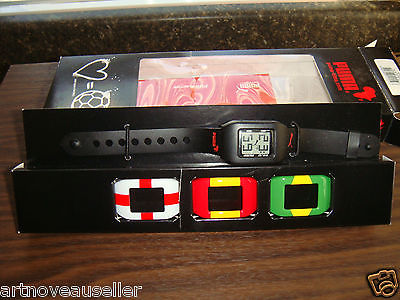
\includegraphics[scale=0.25]{images/ground_truth/1/image_1} & 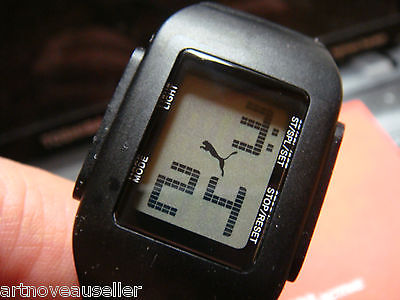
\includegraphics[scale=0.25]{images/ground_truth/1/image_2} & 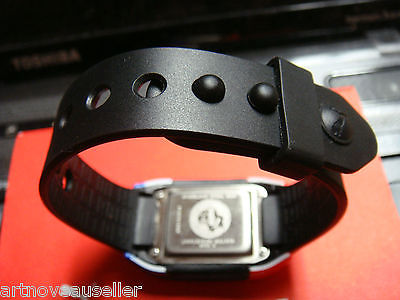
\includegraphics[scale=0.25]{images/ground_truth/1/image_3} \\
	\cline{2-4}
	\multirow{6}{*}{} & Title &  \multicolumn{2}{| p{10cm} |}{NIB 45 EURO \$\$ PUMA SPORT WRISTWATCH SWISS WATCH MOVEMENT LOVE+FOOTBALL} \\
	\cline{2-4}
	\multirow{6}{*}{} & Description &  \multicolumn{2}{| p{10cm} |}{ITEM IS BRAND NEW, FROM THE FIFA WORLD (MUNDIAL) FOOTBALL GAMES. WATCH HAS THREE INTERCHANGEABLE TOP COVER , EACH ONE REPRESENTING THE FLAG OF A TEAM PLAYING AT THE FIFA WORLD (MUNDIAL) FOOTBALL GAME PLUS ONE BLACK COVER IF YOU DON'T WISH TO WEAR THE FLAG COLORS INCLUDED IN THE PACKAGE AS SHOWN IN MY PICTURES. ITEM IS BRAND NEW NEVER USED WITH ORIGINAL BOX PAPERS AND INSTRUCTION ON HOW TO USE THIS WATCH.GREAT GIFT IDEA OR GREAT WATCH FOR THE SPORT LOVERS.ITEM COMES WITH WARRANTY FOR 90 DAYS FROM US AND MANUFACTURER WARRANTY OF 2 YEARS IS INCLUDED IN THE BOX.INSTRUCTIONS ARE IN DUTCH,ENGLISH,FRENCH,ITALIAN, CZECH,GERMAN, PORTUGUESE,SPANISH,HUNGARIAN,CHINESE AND JAPANESE.} \\
	\cline{2-4}
	\multirow{6}{*}{} & Category &  \multicolumn{2}{| p{10cm} |}{Jewelry \& Watches:Watches:Wristwatches} \\
	\cline{2-4}
	\multirow{6}{*}{} & Condition &  \multicolumn{2}{| p{10cm} |}{New with tags} \\
	\cline{2-4}
	\multirow{6}{*}{} & Price &  \multicolumn{2}{| p{10cm} |}{4.99} \\
	\hline \hline
	ID & Image 1 & Image 2 & Image 3 \\
	\hline
	\multirow{6}{*}{2} & 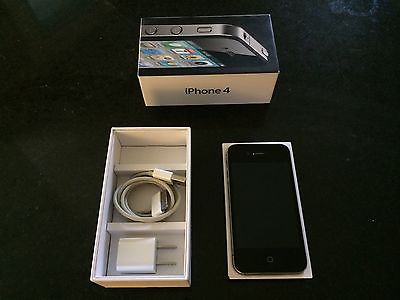
\includegraphics[scale=0.25]{images/ground_truth/2/image_1} & 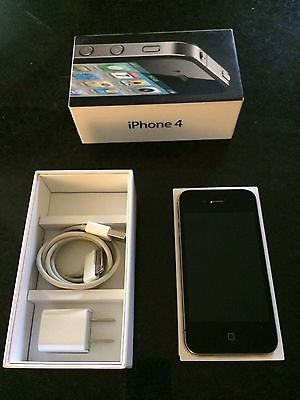
\includegraphics[scale=0.25]{images/ground_truth/2/image_2} & 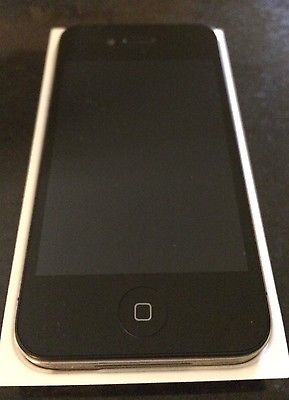
\includegraphics[scale=0.25]{images/ground_truth/2/image_3} \\
	\cline{2-4}
	\multirow{6}{*}{} & Title &  \multicolumn{2}{| p{10cm} |}{Apple iPhone 4 - 16GB - Black (Unlocked) Smartphone} \\
	\cline{2-4}
	\multirow{6}{*}{} & Description &  \multicolumn{2}{| p{10cm} |}{16GB Black iPhone 4, unlocked by carrier. This was an AT\&T phone so it is GSM, can be used internationally. This phone was manufacturer refurbished and then only used for about a week, so it is basically in perfect condition. Includes original packaging, 30-pin USB connector and charger.} \\
	\cline{2-4}
	\multirow{6}{*}{} & Category &  \multicolumn{2}{| p{10cm} |}{Cell Phones \& Accessories:Cell Phones \& Smartphones} \\
	\cline{2-4}
	\multirow{6}{*}{} & Condition &  \multicolumn{2}{| p{10cm} |}{Used} \\
	\cline{2-4}
	\multirow{6}{*}{} & Price &  \multicolumn{2}{| p{10cm} |}{185.0} \\
	\hline \hline
	ID & Image 1 & Image 2 & Image 3 \\
	\hline
	\multirow{6}{*}{3} & 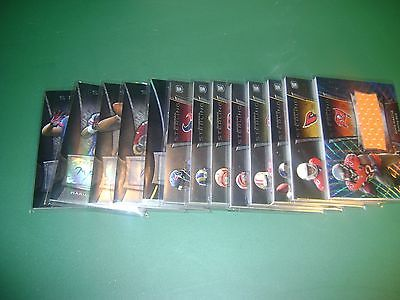
\includegraphics[scale=0.25]{images/ground_truth/3/image_1} & 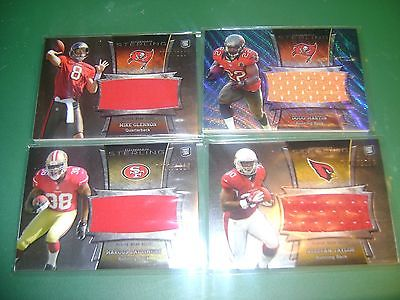
\includegraphics[scale=0.25]{images/ground_truth/3/image_2} & 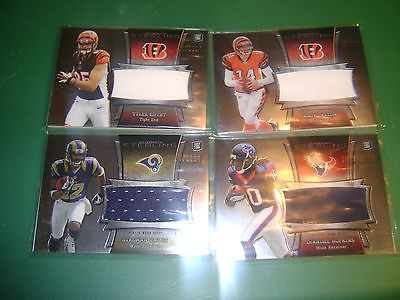
\includegraphics[scale=0.25]{images/ground_truth/3/image_3} \\
	\cline{2-4}
	\multirow{6}{*}{} & Title &  \multicolumn{2}{| p{10cm} |}{Lot of (13) 2013 Bowman Sterling Autograph Auto Relic Jersey Games Used} \\
	\cline{2-4}
	\multirow{6}{*}{} & Description &  \multicolumn{2}{| p{10cm} |}{This is for a 2013 Bowman Sterling Lot of 13 Game Used Relics and Autos. You get the exact cards that you see in the pictures. PLEASE PAY BY PAYPAL WITHIN 24 HOURS OF AUCTIONS END OR ITEM WILL BE RELISTED. S+H IS 3.99 WITH DELIVERY CONFIRMATION PLEASE CHECK OUT MY OTHER AUCTIONS} \\
	\cline{2-4}
	\multirow{6}{*}{} & Category &  \multicolumn{2}{| p{10cm} |}{Sports Mem, Cards \& Fan Shop:Cards:Football} \\
	\cline{2-4}
	\multirow{6}{*}{} & Condition &  \multicolumn{2}{| p{10cm} |}{Brand New} \\
	\cline{2-4}
	\multirow{6}{*}{} & Price &  \multicolumn{2}{| p{10cm} |}{27.0} \\
	\hline \hline
	ID & Image 1 & Image 2 & Image 3 \\
	\hline
	\multirow{6}{*}{4} & 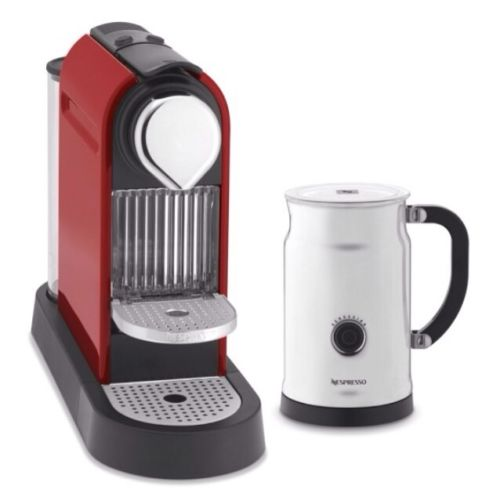
\includegraphics[scale=0.25]{images/ground_truth/4/image_1} & 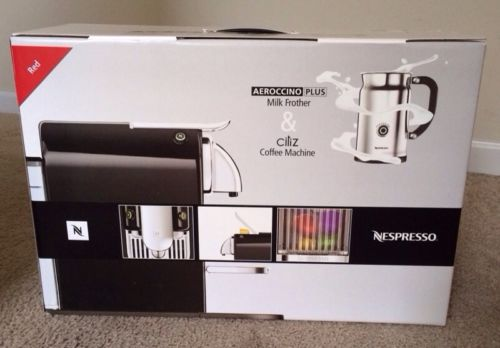
\includegraphics[scale=0.25]{images/ground_truth/4/image_2} & 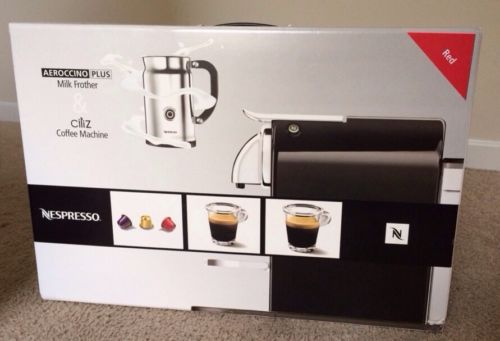
\includegraphics[scale=0.25]{images/ground_truth/4/image_3} \\
	\cline{2-4}
	\multirow{6}{*}{} & Title &  \multicolumn{2}{| p{10cm} |}{Nespresso Aeroccino Plus \& Citiz Coffee Machine {Red}} \\
	\cline{2-4}
	\multirow{6}{*}{} & Description &  \multicolumn{2}{| p{10cm} |}{Nespeesso Aeroccino Plus \& Citiz Coffee Machine Fully automatic brewing and milk frothing in two sleek, compact units. Works exclusively with Nespresso's premium coffee capsules, which are easy to order for delivery within two business days (for details, visit www.nespresso.com). Innovative Thermoblock technology with stainless-steel heating element guarantees precise temperature control. A 19-bar pressure pump ensures maximum extraction of flavor. Adjustable tray accommodates cups of various sizes (from small mug to travel cup). Removable water tank for easy refilling. Energy-save mode gradually reduces power if unit is left on. Includes Aeroccino Plus milk frother, which quickly heats milk for consistently perfect foam. Frother has two whisk attachments and an auto shutoff feature. Espresso maker: ABS plastic housing. 14 1/2" x 5" x 11" high. 34-fl.-oz.-cap. water tank. 10 lb. 1200W. Milk frother: Stainless-steel and plastic construction. 4" diam., 6-3/4" high. 8-oz. cap. 550W. This product is intended for use in the United States and Canada and is built to United States electrical standards. Posted with eBay Mobile} \\
	\cline{2-4}
	\multirow{6}{*}{} & Category &  \multicolumn{2}{| p{10cm} |}{Home \& Garden:Kitchen, Dining \& Bar:Small Kitchen Appliances:Coffee \& Tea Makers:Espresso Machines} \\
	\cline{2-4}
	\multirow{6}{*}{} & Condition &  \multicolumn{2}{| p{10cm} |}{New} \\
	\cline{2-4}
	\multirow{6}{*}{} & Price &  \multicolumn{2}{| p{10cm} |}{201.0} \\
	\hline \hline
	ID & Image 1 & Image 2 & Image 3 \\
	\hline
	\multirow{6}{*}{5} & 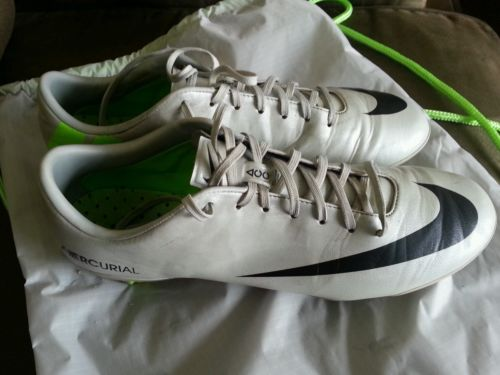
\includegraphics[scale=0.25]{images/ground_truth/5/image_1} & 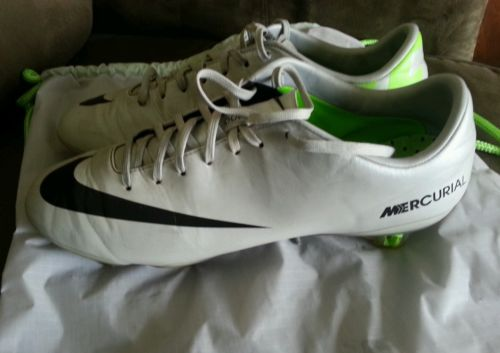
\includegraphics[scale=0.25]{images/ground_truth/5/image_2} & 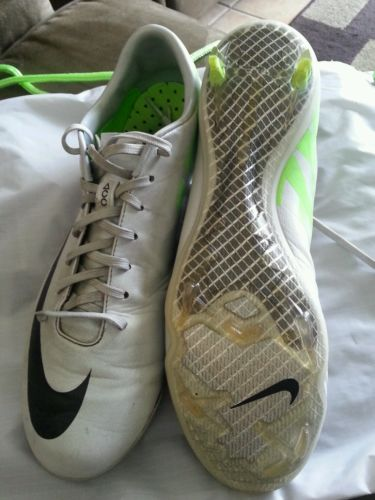
\includegraphics[scale=0.25]{images/ground_truth/5/image_3} \\
	\cline{2-4}
	\multirow{6}{*}{} & Title &  \multicolumn{2}{| p{10cm} |}{Nike Mercurial Vapor IX FG - Soccer Shoes Cleats - Metallic Platinum} \\
	\cline{2-4}
	\multirow{6}{*}{} & Description &  \multicolumn{2}{| p{10cm} |}{This is a pair of used Nike Vapor IX. They come with the string bag. In overall good condition with some signs of use. Clean and no smells. Mens size 7.5. Shipping is \$10.00 and includes tracking. I accept PayPal for payment.} \\
	\cline{2-4}
	\multirow{6}{*}{} & Category &  \multicolumn{2}{| p{10cm} |}{Sporting Goods:Team Sports:Soccer:Clothing, Shoes \& Accessories:Shoes \& Cleats:Men} \\
	\cline{2-4}
	\multirow{6}{*}{} & Condition &  \multicolumn{2}{| p{10cm} |}{Pre-owned} \\
	\cline{2-4}
	\multirow{6}{*}{} & Price &  \multicolumn{2}{| p{10cm} |}{76.99} \\
	\hline \hline
	ID & Image 1 & Image 2 & Image 3 \\
	\hline
	\multirow{6}{*}{6} & 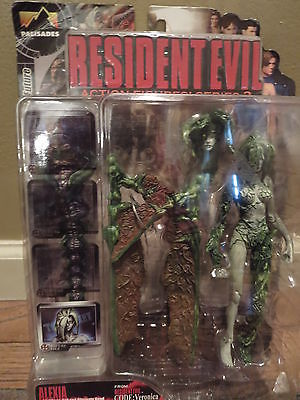
\includegraphics[scale=0.75]{images/ground_truth/6/image_1} & 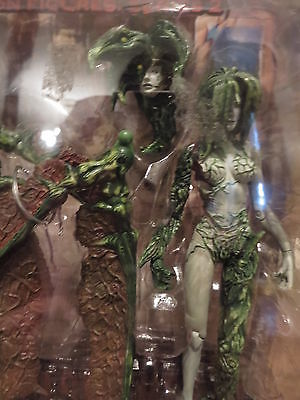
\includegraphics[scale=0.75]{images/ground_truth/6/image_2} & 
\includegraphics[scale=0.75]{images/ground_truth/6/image_3} \\
	\cline{2-4}
	\multirow{6}{*}{} & Title &  \multicolumn{2}{| p{10cm} |}{RARE Series 2 Palisades Resident Evil Code Veronica Alexia Action Figure} \\
	\cline{2-4}
	\multirow{6}{*}{} & Description &  \multicolumn{2}{| p{10cm} |}{This RARE and HARD TO FIND action figure will make and AWESOME collectable for any Resident Evil fan! This specific figure is part of the Resident Evil Code Veronica series. Alexia comes complete with Wings, Tail and Alternate Head to Transform into Alexia III and Logo Base. Great item for any RE fan!!! This item is still in its original packaging, unopened and unused. There is very slight wear around the cardboard edging from years of storage and a little adhesive residue on the plastic, most likely from a price sticker. Overall this item is in excellent condition!} \\
	\cline{2-4}
	\multirow{6}{*}{} & Category &  \multicolumn{2}{| p{10cm} |}{Toys \& Hobbies:Action Figures:TV, Movie \& Video Games} \\
	\cline{2-4}
	\multirow{6}{*}{} & Condition &  \multicolumn{2}{| p{10cm} |}{New} \\
	\cline{2-4}
	\multirow{6}{*}{} & Price &  \multicolumn{2}{| p{10cm} |}{90.0} \\
	\hline \hline
	ID & Image 1 & Image 2 & Image 3 \\
	\hline
	\multirow{6}{*}{7} & 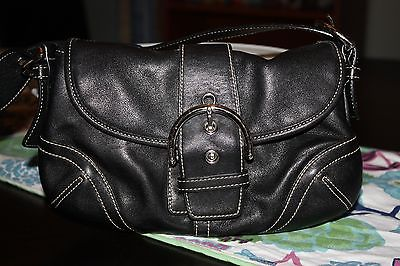
\includegraphics[scale=0.25]{images/ground_truth/7/image_1} & 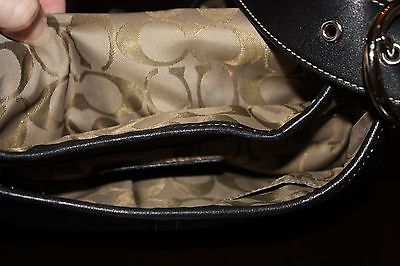
\includegraphics[scale=0.25]{images/ground_truth/7/image_2} & 
\includegraphics[scale=0.25]{images/ground_truth/7/image_3} \\
	\cline{2-4}
	\multirow{6}{*}{} & Title &  \multicolumn{2}{| p{10cm} |}{Black Coach purse leather GUC serial number H050-9247} \\
	\cline{2-4}
	\multirow{6}{*}{} & Description &  \multicolumn{2}{| p{10cm} |}{Pre-owned Black Coach hobo purse. GUC just because I did use it a couple of times. No stains,marks, or tears. Great condition!!!} \\
	\cline{2-4}
	\multirow{6}{*}{} & Category &  \multicolumn{2}{| p{10cm} |}{Clothing, Shoes \& Accessories:Women's Handbags \& Bags:Handbags \& Purses} \\
	\cline{2-4}
	\multirow{6}{*}{} & Condition &  \multicolumn{2}{| p{10cm} |}{Pre-owned} \\
	\cline{2-4}
	\multirow{6}{*}{} & Price &  \multicolumn{2}{| p{10cm} |}{35.0} \\
	\hline
\caption{Ground truth for pure crowdsourcing}
\end{longtable}
\subsection{Tasks workflow}
The macro task of generating an auction on eBay is splited into four simpler micro task:
\begin{itemize}
	\item Generate a title for the auction item based on the provided images of the item
	\item Generate the description of the item
	\item Find the category of auction item
	\item Define a starting price for the auction
\end{itemize}
[Create image of workflow]

\subsection{Task design}
\subsubsection{Title}
\subsubsection{Description}
\subsubsection{Category}
\subsubsection{Price estimation}
Another idea to estimate the starting price is inspired by a German TV game show. The candidate has to predict the cost of an article. After the first guess, the game master answers with 'higher' or 'lower' until the right guess occur or the time is running out. If the player finds out the correct price then she/he will win the object.  
The idea of the show is modified to implement a game with a purpose, similar to the ESP game project \cite{esp}. The general procedure of the game is the following: 
\begin{enumerate}
	\item The system waits until two independent players are connected and ready to play 
	\item A few pictures, title and description of the article are displayed and the players had to read them first 
	\item Then the game starts and a first guess of the price will be shown by the system 
	\item Both users have to decide if the real price is higher or lower than the displayed one 
	\item Dependent on the previous response, the system will present a higher or lower price until the countdown is expired or there are no guesses left 
	\item The players will receive a score dependent on the difference of the price estimation. A smaller difference leads to a higher score, a higher one to a lower score 
\end{enumerate}
The first guess of the system will be the mean value \( \mu \) of a large number of sold items on eBay. The value can be determined by the eBay API. The guessing structure will be implemented as a directed binary tree. The root node represents the mean value and every following child node will have a lower (left child) \( v_l \) or higher (right child) value  \( v_r \), determined by the value of the parent node  \( v_p \) and the depth  \( d \) of the tree. The following formula calculates the values  of the nodes: 
\begin{equation}
v_l(v_p,d) = v_p - \frac{\mu}{2^d}
\end{equation}
\begin{equation}
v_r(v_p,d) = v_p + \frac{\mu}{2^d}
\end{equation}
The leafs are integer values which can't be divided by two and represents the final guess of a player. If the time is up and the guesser doesn't reach a leaf node, the value of the actual node is taken. 
The score of the price prediction is determined by a scoring function \( s \), where \( x_1 \) and \( x_2 \) are the price estimations of player 1 and 2.
\begin{equation}
s(x_1,x_2) = 1 - |\varphi(x_1) - \varphi(x_2)|
\end{equation}
The function \( \varphi \) is responsible to normalise the estimations (interval from 0 to 1).
\begin{equation}
\varphi(x) = \frac{x}{2\mu}
\end{equation}
The function is also used to weight the different estimations for the same product. If \( n \) rounds are played for a given object, the final price \( t \) is calculated:
\begin{equation}
t = \frac{1}{\sum_{k=1}^{n} s(x_{k1},x_{k2})}\left(\sum_{i=1}^{n} s(x_{i1},x_{i2})\frac{x_{i1}+x_{i2}}{2}\right)
\end{equation}
The reliability \( r \) of the price estimation is the mean score of all played games for the same object:
\begin{equation}
r = \frac{1}{n}\left(\sum_{i=1}^{n} s(x_{i1},x_{i2})\right)
\end{equation}

\section{Hybrid approach}
\subsection{Ground truth}
A lot of sold items were collected by the help of the eBay API. The used methods were the same as in the prior ground truth generation (Chapter x). After all the necessary data were collected, the Python script splits the data shuffled into a training and test set. The training set contains of 70 percent of the whole data. All the consecutively steps (data analysis, feature reduction) will use the training set until the performance of a classifier will be proved on the test set. The ground truth was generated for three different item types:
\begin{table}[h!]
	\begin{center}
	\begin{tabular}{| p{5cm} | l | l | l |}
		\hline
		Item type & Total number of auctions & Size of training set & Size of test set \\
		\hline
		Apple iPhone & 2299 & 1609 & 690 \\
		\hline
		Hot Wheels Cars, 1:64, Ford Mustang & & & \\
		\hline
		Sony Playstation & & & \\
		\hline
	\end{tabular}
	\end{center}
	\caption{}
\end{table}
\subsection{Tasks workflow}
\subsection{Task design}
\subsubsection{Title}
\paragraph{Finding}
\subparagraph{Overview}
\begin{table}[h!]
	\begin{center}
	\begin{tabular}{| l | p{10cm} |}
		\hline
		Title & Give auction items a title based on several images \\
		\hline
		Description & Take a look at three pictures of an auction item and write down a predicative title \\
		\hline
		Keywords & image, description, picture, item, title, auction \\
		\hline
		Reward & 0.05 USD \\
		\hline
		Lifetime & 7 Days \\
		\hline
		Assignment duration & 30 minutes \\
		\hline
		Assignments & 3 \\
		\hline
		Qualification requirement & Location is US \\
		\hline
	\end{tabular}
	\end{center}
	\caption{}
\end{table}
\subparagraph{Question 1}
The goal of the requester of the HIT is to generate eBay auctions by MTurk workers based on images of the item.\\
Instructions: Write a title which describes the item(s) on the pictures, inside the empty text field below and keep in mind the following remarks:
\begin{itemize}
	\item Use descriptive keywords to clearly and accurately convey what you're seeing. You're allowed up to 80 characters, but you don't need to use them all
	\item Include the item's brand name, artist, or designer if possible
	\item Include item specifics. For example, include size, color, condition, and model number if possible
	\item Use correct spelling
	\item Don't use all caps
	\item Take a look at the provided example 
\end{itemize}
\paragraph{Voting}
\subparagraph{Overview}
\begin{table}[h!]
	\begin{center}
	\begin{tabular}{| l | p{10cm} |}
		\hline
		Title & Vote for an auction item title based on several images \\
		\hline
		Description & Take a look at three pictures of an auction item and select a title \\
		\hline
		Keywords & image, description, picture, item, title, vote, auction \\
		\hline
		Reward & 0.02 USD \\
		\hline
		Lifetime & 7 Days \\
		\hline
		Assignment duration & 30 minutes \\
		\hline
		Assignments & 3 \\
		\hline
		Qualification requirement & Location is US \\
		\hline
	\end{tabular}
	\end{center}
	\caption{}
\end{table}
\subparagraph{Question 1}
The goal of the requester of the HIT is to generate eBay auctions by MTurk workers based on images of the item.\\
Instructions: Select the title which describes clearly and accurately the auction item(s) on the pictures. Keep in mind the following restrictions:
\begin{itemize}
	\item Do not select a title which contains wrong information
	\item Do not select a title which has spelling mistakes (e.g. Sny Playstation 4, black)
	\item Do not select a title which is written in capital letters (e.g. SONY PLAYSTATION 4, BLACK)
\end{itemize}
If you think that no title is suitable for the item(s) then select None. 
\subparagraph{Question 2}
Give reasons for your selection:
\begin{itemize}
	\item Explain why the selected title is the best description of the item(s) on the pictures
	\item Explain the deficits of the non-selected titles (e.g. incorrect information)
\end{itemize}
Attention: Only HITs with meaningful reasoning will be approved 
\subsubsection{Description}
\subsubsection{Category}
\subsubsection{Price estimation}
\subsection{Pre-processing}
\subsection{Feature extraction}
\subsubsection{Item Specific Features}
\paragraph{Apple iPhone}
The iPhone made by Apple is available in eight models. The first generation was released in 2007, the last model 5s in 2013. Every model comes with different storage sizes (from 8GB to 64GB). The values for the condition property on eBay depend on the corresponding item category. All the values are nominal and will be converted to numerical.
\begin{table}[h!]
	\begin{center}
	\begin{tabular}{| l | p{5cm} | p{4cm} | l | l |}
		\hline
		Name & Description & Values & Range & Data type \\
		\hline
		Model & The model of the iPhone where 0 is the oldest generation and 7 the newest & 1st, 3G, 3GS, 4, 4S, 5, 5C, 5S & [0, 7] & Integer \\
		\hline
		Storage & The size of the storage of the smartphone & 8GB, 16GB, 32GB, 64GB & [1, 4] & Integer \\
		\hline
		Condition & The condition of the iPhone & New, New other, Manufacturer refurbished, Seller refurbished, Used, For parts or not working & [1, 6] & Integer \\
		\hline
	\end{tabular}
	\end{center}
	\caption{}
\end{table}
\subsubsection{Auction Specific Features}
The auction itself is described by the features in this section. The list contains some timing and shipping information. Also the number of pictures and the description length could have an influence to the result of the auction. All values are numerical.
\begin{table}[h!]
	\begin{center}
	\begin{tabular}{| l | p{5cm} | l | l | l |}
		\hline
		Name & Description &  Range & Data type \\
		\hline
		Duration & The duration of the auction in days & {1, 2, 3, 7, 10} & Integer \\
		\hline
		Number of pictures & Number of pictures attached to the auction & [1, 12] & Integer \\
		\hline
		Length of description & Length of the item description & [0, 500'000] & Integer \\
		\hline
		End weekday & The last weekday of the auction duration & [1, 7] & Integer \\
		\hline
		Start weekday & The weekday of the creation date & [1, 7] & Integer \\
		\hline
		End hour & At what hour the auction was ended & [0, 23] & Integer \\
		\hline
		Global shipping & The item will be shipped over the whole world or not & {0, 1} & Boolean \\
		\hline
		Shipping locations & The number of countries where the item will be shipped & [0, 249] & Integer \\
		\hline
		Shipping type & Specifies the calculation of the shipping costs & [0, 7] & Integer \\
		\hline
		Returns accepted & If the buyer can return the item or not & {0, 1} & Boolean \\
		\hline
		Handling time & How many days will it take until the item is put in the mail once the seller receive payment & {1, 2, 3, 4, 5, 10, 15, 20} & Integer \\
		\hline
	\end{tabular}
	\end{center}
	\caption{}
\end{table}
\subsubsection{Seller Specific Features}
These features characterise the seller who created the auction. Every user on eBay has the possibility to give a positive, neutral or negative feedback after every transaction. The rating system awards stars with twelve different colors for trustful sellers. After ten positive feedbacks the user receives a yellow star for example. Therefore, the nominal value has to be converted to an integer.
\begin{table}[h!]
	\begin{center}
	\begin{tabular}{| l | l | l | l | l |}
		\hline
		Name & Description &  Range & Data type \\
		\hline
		Seller rating & Percentage of positive feedbacks & [0, 100] & Float \\
		\hline
		Seller rating count & Number of positive minus negative buyer feedbacks & [0, 12] & Integer \\
		\hline
	\end{tabular}
	\end{center}
	\caption{}
\end{table}
\subsection{Feature selection}
\subsection{Classifiers}


\chapter{Evaluation}
\label{chap:evaluation}
\section{Pure approach}
\subsection{Overall Performance}
After all the necessary content was created by the crowd, the evaluation was done by comparing the ground truth with the generated information. The evaluation task presented the fields title, description and category to the workers. They had to decide which auction description is the best one in their opinion. The result is illustrated in figure \ref{crowdsourcing_eval}. The commission approach got a majority of the votes with 57.14\%. The table received all five votes from the crowd. The ground truth contains unnecessary information and looks like a scam, is the statement of the participants.\\
\begin{figure}
\centering
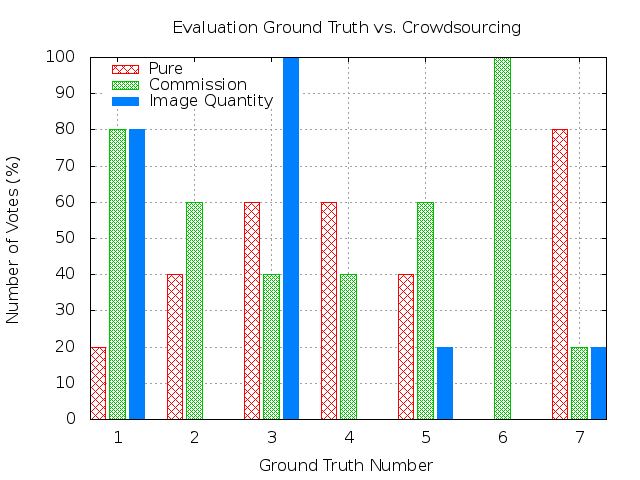
\includegraphics[scale=0.55]{images/plots/crowdsourcing/plot_evaluation_all.png}
\caption{Evaluation of Ground Truth vs. Crowdsourcing}
\label{crowdsourcing_eval}
\end{figure}
The workers had the possibility to reason their decision. They motivate their votes as follows: 
\begin{itemize}
	\item Higher value of information 
	\item Professionalism 
	\item Hidden information are given (e.g. size of the cleats, size of the smartphone storage) 
	\item The description is clear, short and to the point 
	\item Authenticity of the article 
	\item Grammatical issues 
\end{itemize}

\subsection{Title}
The length of the title (Figure \ref{crowdsourcing_title_length}) increases if the task contains all available pictures of the item. This setup produced an average title length of 64 characters. The other experiments have an average of 50 for the standard design and 48 for a promised commission. The median value shows almost the same ranking except the additional reward in form of a commission generates more characters than the standard configuration. The item without a brand was described by a title with 37 characters. The length doesn't say anything about the quality of the title, but it indicates the influence of the different task settings. The usage of natural language processing tools could help to get more information about the quality, but this would be outside the scope of the thesis.
\begin{figure}
\centering
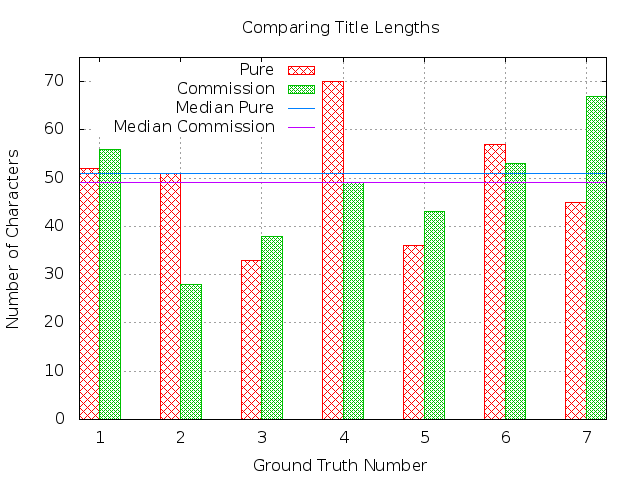
\includegraphics[scale=0.55]{images/plots/crowdsourcing/plot_title_length.png}
\caption{Evaluation of Title Lengths}
\label{crowdsourcing_title_length}
\end{figure} 

After the creation of the titles, the workers had to select the final one for each item. They justify their selections as follows:
\begin{itemize}
	\item Amount of details 
	\item Attracts more attention 
	\item Research on eBay produces better results for the title 
	\item Experiences with online auctions 
	\item Wrong information 
	\item Too long 
\end{itemize}

\subsection{Description}
The same measurements as for the title were done for the description (Figure \ref{crowdsourcing_desc_length}). The general task design achieved the highest average length (467 chars), but it contains an outlier with 1706 characters for the ground truth item number 5. The worker copied an item description from the website of the producer. More images doesn't conclude to a longer description, because the average length of these titles is 281. An extra reward leads to 455 characters, but has the highest median of 572. The numeric parameter is more robust to outliers. The other setups follow by 307 (Commission) and 238 (Pure). The non-branded item realise a length of 240 characters which is equal to the median of the branded items. Therefore, the workers are able to write descriptions of equal length regardless of which item type (branded/non-branded) was presented to them.
\begin{figure}
\centering
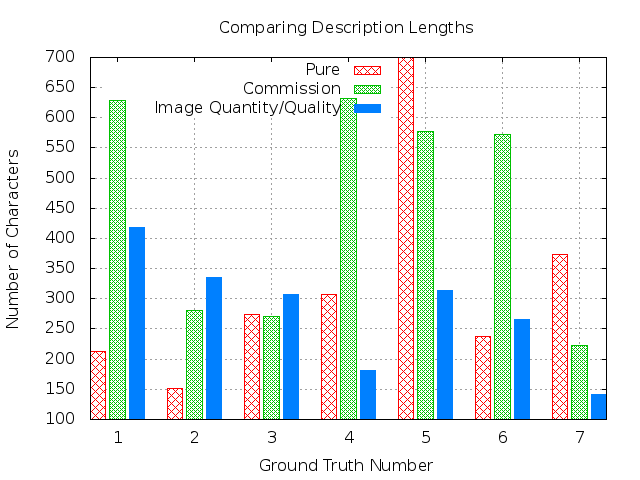
\includegraphics[scale=0.55]{images/plots/crowdsourcing/plot_description_length.png}
\caption{Evaluation of Description Lengths}
\label{crowdsourcing_desc_length}
\end{figure}

\subsection{Category}
Most of the workers submitted only the main category and not the complete hierarchy with main and sub categories. For the football trading cards they wrote ''Sports Mem, Cards \& Fan Shop'' instead of ''Sports Mem, Cards \& Fan Shop:Cards:Football'', for example. One reason could be that the instructions weren't clear and precise enough. Also the desired format of the input wasn't mentioned. An improved task design will result in more accurate outputs.
\subsection{Price Estimation}
To evaluate the accuracy of the price estimations (Figure \ref{crowdsourcing_price_pred}), the root mean squared error (RMSE) was used. It is frequently used to measure the quality of predictions. The true values are the end prices from the ground truth. If the workers have the actual market price of the item at one's disposal then they predict the price best with an average RMSE of 51.46 USD. The experiment with the commission ranked just behind with 58.55 USD, the others appear with 81.75 (Pure) and 89.89 (Image quantity/quality) at the end of the ranking. The tested item without a brand has a RMSE of 278.62 USD which indicates the challenge of the price prediction for generic things.\\
The estimation errors can be explained by different observations. The size of the smartphone storage isn't given. The price difference of an iPhone 5S with 32GB and 64GB is about 100 dollars. The football trading cards are difficult to estimate, because most of the workers don't know the football players and cannot asses the rarity or popularity of them. The football boot model is available in different versions. The original one and the cheaper replica. The action figure is rare and no other auctions are available to compare with. The women handbag could be a fake or an original Coach\footnote{http://www.coach.com} bag.
\begin{figure}
\centering
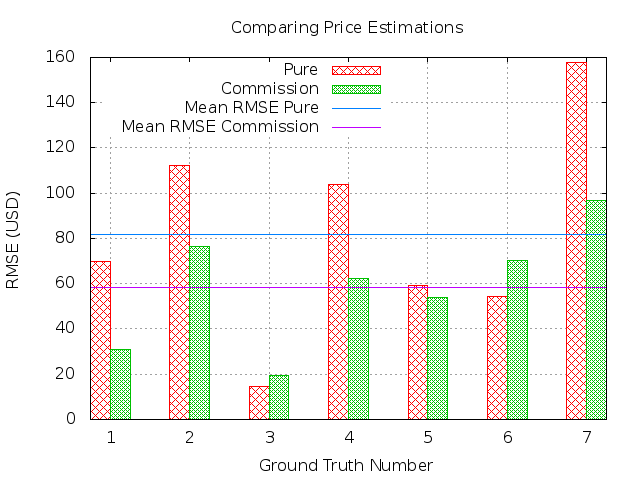
\includegraphics[scale=0.55]{images/plots/crowdsourcing/plot_price_rmse.png}
\caption{Price Prediction Quality}
\label{crowdsourcing_price_pred}
\end{figure}
Under/Over estimations
\begin{figure}
\centering
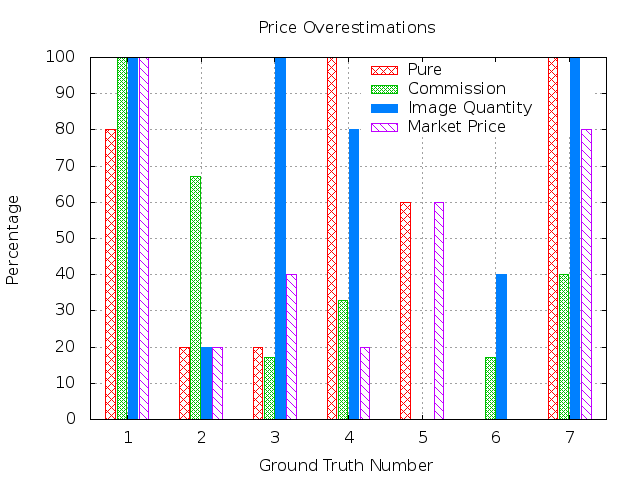
\includegraphics[scale=0.55]{images/plots/crowdsourcing/plot_price_overestimation.png}
\caption{Price Overestimations}
\label{crowdsourcing_price_overestimations}
\end{figure}
\subsection{Variations}
\subsubsection{Commission}
The ground truth items 1 and 3 received a majority of the votes from the crowd. The commissions were paid manually using the web interface of the Amazon Mechanical Turk web service. The value of the bonus has to be shortened to two digits after the point and rounded up to \$0.01, because of some restrictions of MTurk. The bonus aggregates to \$1.48 for both auctions. The worker received also an additional message: \\
''Dear worker, \\

You receive a commission (0.25\% of the end price) as bonus payment for your work. The end price of the eBay online auction was \$27.''
\begin{table}[h!]
	\begin{center}
	\begin{tabular}{| p{1cm} | p{1.5cm} | p{3cm} | p{1.5cm} | p{1.5cm} | p{3.5cm} |}
		\hline
		Ground truth number & End price (USD) & Task & Percentage & Bonus (USD) & Worker ID \\
		\hline
		1 & 4.99 & Title (Finding) & 0.25\% & 0.01 & A3HE1W5T6QO03X \\
		\hline
		1 & 4.99 & Title (Voting) & 0.1\% & 0.01 & A3N7O1NOBGX6U7 \\
		\hline
		1 & 4.99 & Title (Voting) & 0.1\% & 0.01 & A1DK26QAO4OOMQ \\
		\hline
		1 & 4.99 & Description (Improving) & 1\% & 0.05 & A2Y9ZNZ0F24GHB \\
		\hline
		1 & 4.99 & Description (Voting) & 0.05\% & 0.01 & A2FF8HA1OWKS83 \\
		\hline
		1 & 4.99 & Description (Voting) & 0.05\% & 0.01 & AJAOE1PSNKGUE \\
		\hline
		1 & 4.99 & Category & 0.25\% & 0.01 & A2ZT4MTMEVSLB9 \\
		\hline
		1 & 4.99 & Category & 0.25\% & 0.01 & A220ED0LJITW5I \\
		\hline
		1 & 4.99 & Category & 0.25\% & 0.01 & A2V8WJXA0USMZ \\
		\hline
		1 & 4.99 & Price & 0.5\% & 0.02 & A3L99RGPK6FZGH \\
		\hline
		3 & 27 & Title (Finding) & 0.25\% & 0.06 & A23BCMQN9ZU97B \\
		\hline
		3 & 27 & Title (Voting) & 0.1\% & 0.02 & A3N7O1NOBGX6U7 \\
		\hline
		3 & 27 & Title (Voting) & 0.1\% & 0.02 & A3I4BYP4DUC475 \\
		\hline
		3 & 27 & Description (Improving) & 1\% & 0.27 & A1IA4CST74I1Q8 \\
		\hline
		3 & 27 & Description (Voting) & 0.05\% & 0.01 & A3K77RSYXLLUQL \\
		\hline
		3 & 27 & Description (Voting) & 0.05\% & 0.01 & A25F7BNXEN8I5X \\
		\hline
		3 & 27 & Category & 0.25\% & 0.06 & A2ZT4MTMEVSLB9 \\
		\hline
		3 & 27 & Category & 0.25\% & 0.06 & A220ED0LJITW5I \\
		\hline
		3 & 27 & Category & 0.25\% & 0.06 & A2V8WJXA0USMZ \\
		\hline
		3 & 27 & Price & 0.5\% & 0.13 & A3L99RGPK6FZGH \\
		\hline
	\end{tabular}
	\end{center}
	\caption{}
\end{table}



 

\section{Hybrid approach}
The Random Forest approach shows the best performance over all three item categories independent of classification or regression (Figure). The accuracy of the classifier depends also on the item category. The RFC assign every third input to the right Sony Playstation price class. The plot of the mean absolute error (MAE, Figure) assured the strength of the classifier and visualise how far away the predictions are in average. kNN has an error of about four classes for the iPhone category, one class has a range of 25 USD. The comparison between the human-based and the machine-based prediction indicates that the crowd can't be as accurate as a machine. The lowest RMSE of the ground truth item number 2 (Apple iPhone) is \$76.32. Two machine learning algorithms have a smaller error (Figure). 
The normalised confusion matrix (Figure) of the iPhone classifiers illustrates the distribution of the assignments. The origin is located at the left top position, the x-axis represents the truth-values and the y-axis the values assigned by the classifier. The values were normalised per row. A perfect classifier would produce a diagonal which contains only ones. 
The scatter plot (Figure) is another way to visualise the relations between the truth and predicted values. The criteria of a perfect classifier are the same as for the confusion matrix. 
The same plots for the other categories and the exact accuracies/RMSEs/MAEs are enumerated in the appendix section (Reference).
\begin{figure}
\centering
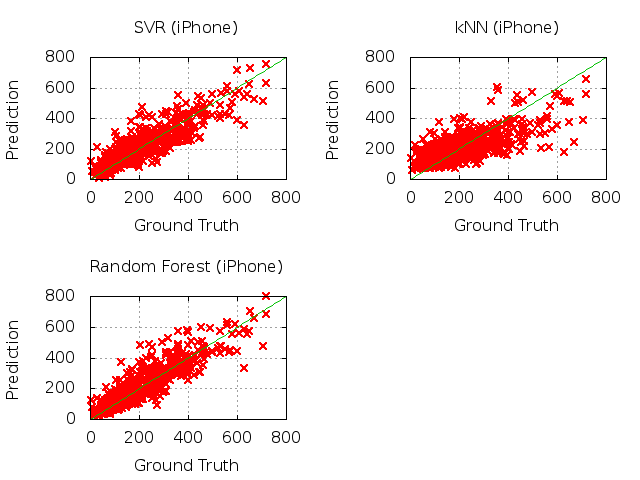
\includegraphics[scale=0.55]{images/plots/machine_learning/iphone/true_pred_iphone.png}
\caption{Scatter plot truth vs. prediction (iPhone)}
\label{truth_predict_iphone}
\end{figure}
\begin{figure}
\centering
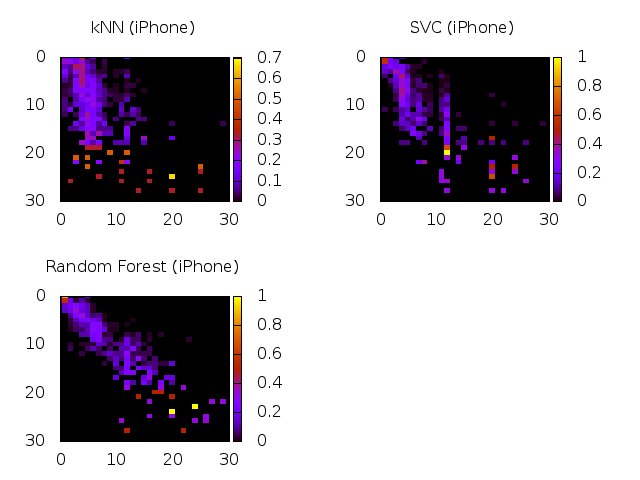
\includegraphics[scale=0.55]{images/plots/machine_learning/iphone/conf_mat_iphone.png}
\caption{Time/Error Function}
\label{crowdsourcing_desc_length}
\end{figure}

\begin{figure}
\centering
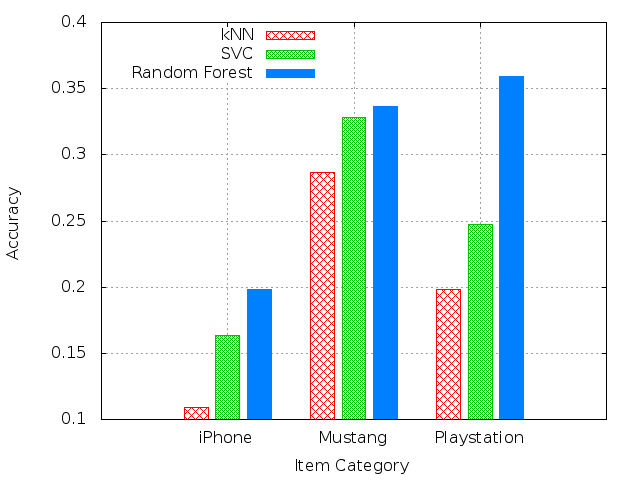
\includegraphics[scale=0.55]{images/plots/machine_learning/plot_price_classification_acc.png}
\caption{Time/Error Function}
\label{crowdsourcing_desc_length}
\end{figure}
\begin{figure}
\centering
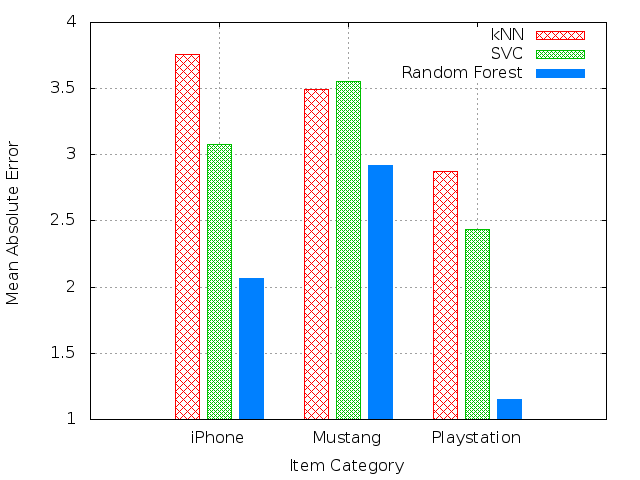
\includegraphics[scale=0.55]{images/plots/machine_learning/plot_price_classification_mae.png}
\caption{Time/Error Function}
\label{crowdsourcing_desc_length}
\end{figure}

\begin{figure}
\centering
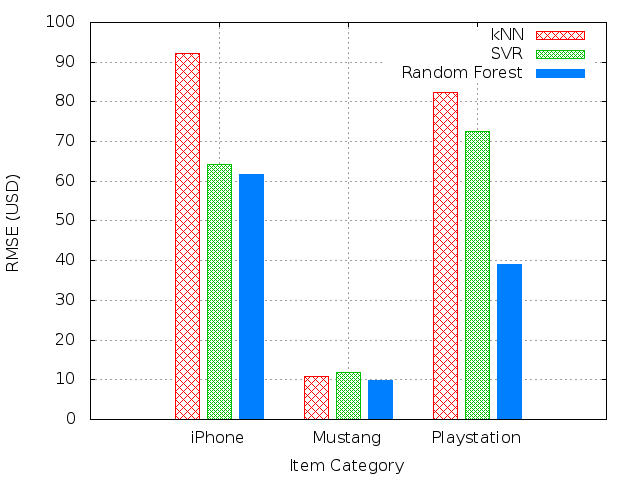
\includegraphics[scale=0.55]{images/plots/machine_learning/plot_price_regression_rmse.png}
\caption{Time/Error Function}
\label{crowdsourcing_desc_length}
\end{figure}





\chapter{Conclusion}
\label{chap:conclusion}
\section{Future work}
\subsection{Google Reverse Image Search}
Some tests during the first phase of the thesis has shown that the reverse Google image search doesn't return reliable results for all types of items. But if the search algorithm find websites which contain information about the item then the application should extract the relevant facts in a certain way. Some experiments should be done and the possibilities of the API should be investigated in the future. 
\subsection{Main Image Selection}
The workers have to decide which of the available images give the best r\'{e}sum\'{e} of the product. If the application should publish the auction on eBay in the future then a representing image of the item has to be determined. 
\subsection{Fully Automated Application}
The creation, administration and evaluation of every subtask is done manually at the moment. The final product can be a mobile application and/or a web service which manages the whole process. The user will take some pictures of the item and upload the data to the server. Then he has to provide some auction specific information (duration, shipping details) and the software will create the auction after all missing inputs are generated by the crowd. Different pricing strategies can be selected. The estimated price can be used as the starting price or the price can be reduced by a predefined percentage rate. 
\subsection{Price Estimation Game}
Another idea to estimate the starting price is inspired by a German TV game show. The candidate has to predict the cost of an article. After the first guess, the game master answers with 'higher' or 'lower' until the right guess occur or the time is running out. If the player finds out the correct price then she/he will win the object.  
The idea of the show is modified to implement a game with a purpose, similar to the ESP game project \cite{esp}. The general procedure of the game is the following: 
\begin{enumerate}
	\item The system waits until two independent players are connected and ready to play 
	\item A few pictures, title and description of the article are displayed and the players had to read them first 
	\item Then the game starts and a first guess of the price will be shown by the system 
	\item Both users have to decide if the real price is higher or lower than the displayed one 
	\item Dependent on the previous response, the system will present a higher or lower price until the countdown is expired or there are no guesses left 
	\item The players will receive a score dependent on the difference of the price estimation. A smaller difference leads to a higher score, a higher one to a lower score 
\end{enumerate}
The first guess of the system will be the mean value \( \mu \) of a large number of sold items on eBay. The value can be determined by the eBay API. The guessing structure will be implemented as a directed binary tree. The root node represents the mean value and every following child node will have a lower (left child) \( v_l \) or higher (right child) value  \( v_r \), determined by the value of the parent node  \( v_p \) and the depth  \( d \) of the tree. The following formula calculates the values  of the nodes: 
\begin{equation}
v_l(v_p,d) = v_p - \frac{\mu}{2^d}
\end{equation}
\begin{equation}
v_r(v_p,d) = v_p + \frac{\mu}{2^d}
\end{equation}
The leafs are integer values which can't be divided by two and represents the final guess of a player. If the time is up and the guesser doesn't reach a leaf node, the value of the actual node is taken. 
The score of the price prediction is determined by a scoring function \( s \), where \( x_1 \) and \( x_2 \) are the price estimations of player 1 and 2.
\begin{equation}
s(x_1,x_2) = 1 - |\varphi(x_1) - \varphi(x_2)|
\end{equation}
The function \( \varphi \) is responsible to normalise the estimations (interval from 0 to 1).
\begin{equation}
\varphi(x) = \frac{x}{2\mu}
\end{equation}
The function is also used to weight the different estimations for the same product. If \( n \) rounds are played for a given object, the final price \( t \) is calculated:
\begin{equation}
t = \frac{1}{\sum_{k=1}^{n} s(x_{k1},x_{k2})}\left(\sum_{i=1}^{n} s(x_{i1},x_{i2})\frac{x_{i1}+x_{i2}}{2}\right)
\end{equation}
The reliability \( r \) of the price estimation is the mean score of all played games for the same object:
\begin{equation}
r = \frac{1}{n}\left(\sum_{i=1}^{n} s(x_{i1},x_{i2})\right)
\end{equation}

\section{Discussion}
\subsection{Pros}
Workers are impartial and enumerate the facts of the item based on the pictures. They don't try to write a sales text. The provided photos aren't ideal to describe the peculiarities of the item. The worker has no chance to mention the storage size of a smartphone if no screenshot of the system properties is given. If the input images. The participants of the price task have fun to guess the most accurate price. This fact has a positive influence to the prediction results. 
\subsection{Cons}
Workers are lazy and minimalist. They copy item descriptions from the websites of the producers and take the first found price of sale for the estimation. The prior goal is to maximise the hourly wage and not to commit high quality content. The owner of the items only knows about small defects and the peculiarities of the item. This important information is missing in the final description and doesn't allow to create an accurate public sale. The spelling of the written descriptions is improvable.


\clearpage

\selectlanguage{english}
\bibliographystyle{bib/custom}
\bibliography{bib/references}
\newpage
\begin{appendices}
\chapter{Ground Truth}
\section{Basic Items}
\lstset{caption={}}
\begin{longtable}{| l | l | l | l |}
	\hline
	ID & Image 1 & Image 2 & Image 3 \\
	\hline
	\multirow{6}{*}{1} & 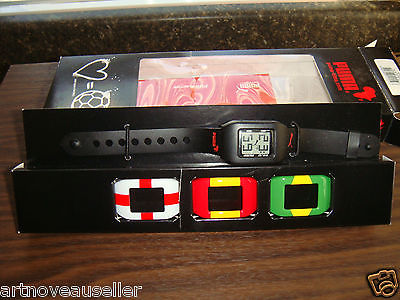
\includegraphics[scale=0.25]{images/ground_truth/1/image_1} & 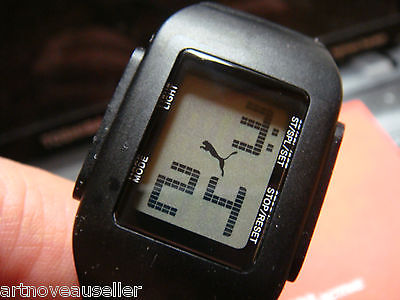
\includegraphics[scale=0.25]{images/ground_truth/1/image_2} & 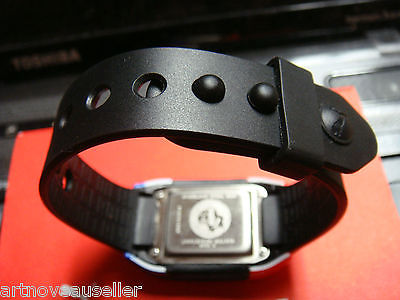
\includegraphics[scale=0.25]{images/ground_truth/1/image_3} \\
	\cline{2-4}
	\multirow{6}{*}{} & Title &  \multicolumn{2}{| p{10cm} |}{NIB 45 EURO \$\$ PUMA SPORT WRISTWATCH SWISS WATCH MOVEMENT LOVE+FOOTBALL} \\
	\cline{2-4}
	\multirow{6}{*}{} & Description &  \multicolumn{2}{| p{10cm} |}{ITEM IS BRAND NEW, FROM THE FIFA WORLD (MUNDIAL) FOOTBALL GAMES. WATCH HAS THREE INTERCHANGEABLE TOP COVER , EACH ONE REPRESENTING THE FLAG OF A TEAM PLAYING AT THE FIFA WORLD (MUNDIAL) FOOTBALL GAME PLUS ONE BLACK COVER IF YOU DON'T WISH TO WEAR THE FLAG COLORS INCLUDED IN THE PACKAGE AS SHOWN IN MY PICTURES. ITEM IS BRAND NEW NEVER USED WITH ORIGINAL BOX PAPERS AND INSTRUCTION ON HOW TO USE THIS WATCH.GREAT GIFT IDEA OR GREAT WATCH FOR THE SPORT LOVERS.ITEM COMES WITH WARRANTY FOR 90 DAYS FROM US AND MANUFACTURER WARRANTY OF 2 YEARS IS INCLUDED IN THE BOX.INSTRUCTIONS ARE IN DUTCH,ENGLISH,FRENCH,ITALIAN, CZECH,GERMAN, PORTUGUESE,SPANISH,HUNGARIAN,CHINESE AND JAPANESE.} \\
	\cline{2-4}
	\multirow{6}{*}{} & Category &  \multicolumn{2}{| p{10cm} |}{Jewelry \& Watches:Watches:Wristwatches} \\
	\cline{2-4}
	\multirow{6}{*}{} & Condition &  \multicolumn{2}{| p{10cm} |}{New with tags} \\
	\cline{2-4}
	\multirow{6}{*}{} & Price &  \multicolumn{2}{| p{10cm} |}{4.99} \\
	\hline \hline
	ID & Image 1 & Image 2 & Image 3 \\
	\hline
	\multirow{6}{*}{2} & 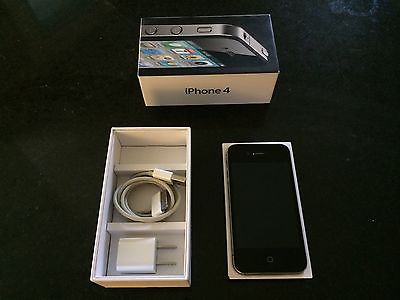
\includegraphics[scale=0.25]{images/ground_truth/2/image_1} & 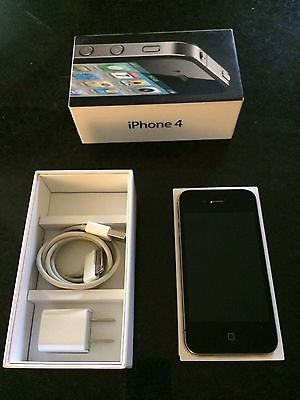
\includegraphics[scale=0.25]{images/ground_truth/2/image_2} & 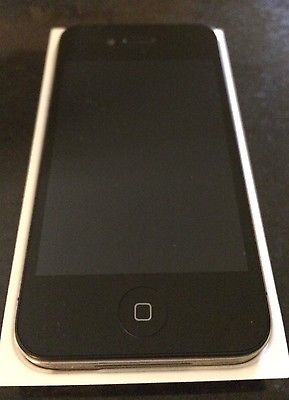
\includegraphics[scale=0.25]{images/ground_truth/2/image_3} \\
	\cline{2-4}
	\multirow{6}{*}{} & Title &  \multicolumn{2}{| p{10cm} |}{Apple iPhone 4 - 16GB - Black (Unlocked) Smartphone} \\
	\cline{2-4}
	\multirow{6}{*}{} & Description &  \multicolumn{2}{| p{10cm} |}{16GB Black iPhone 4, unlocked by carrier. This was an AT\&T phone so it is GSM, can be used internationally. This phone was manufacturer refurbished and then only used for about a week, so it is basically in perfect condition. Includes original packaging, 30-pin USB connector and charger.} \\
	\cline{2-4}
	\multirow{6}{*}{} & Category &  \multicolumn{2}{| p{10cm} |}{Cell Phones \& Accessories:Cell Phones \& Smartphones} \\
	\cline{2-4}
	\multirow{6}{*}{} & Condition &  \multicolumn{2}{| p{10cm} |}{Used} \\
	\cline{2-4}
	\multirow{6}{*}{} & Price &  \multicolumn{2}{| p{10cm} |}{185.0} \\
	\hline \hline
	ID & Image 1 & Image 2 & Image 3 \\
	\hline
	\multirow{6}{*}{3} & 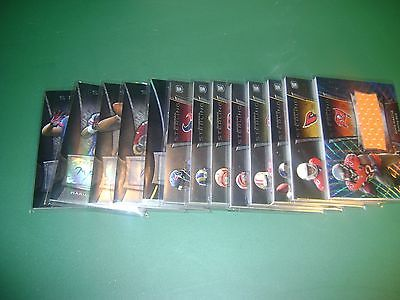
\includegraphics[scale=0.25]{images/ground_truth/3/image_1} & 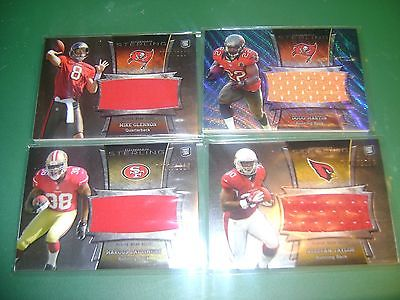
\includegraphics[scale=0.25]{images/ground_truth/3/image_2} & 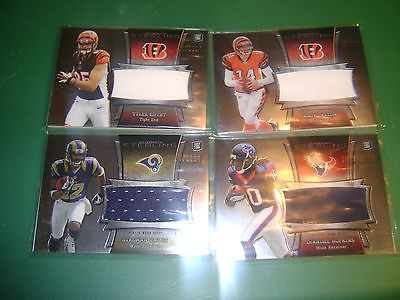
\includegraphics[scale=0.25]{images/ground_truth/3/image_3} \\
	\cline{2-4}
	\multirow{6}{*}{} & Title &  \multicolumn{2}{| p{10cm} |}{Lot of (13) 2013 Bowman Sterling Autograph Auto Relic Jersey Games Used} \\
	\cline{2-4}
	\multirow{6}{*}{} & Description &  \multicolumn{2}{| p{10cm} |}{This is for a 2013 Bowman Sterling Lot of 13 Game Used Relics and Autos. You get the exact cards that you see in the pictures. PLEASE PAY BY PAYPAL WITHIN 24 HOURS OF AUCTIONS END OR ITEM WILL BE RELISTED. S+H IS 3.99 WITH DELIVERY CONFIRMATION PLEASE CHECK OUT MY OTHER AUCTIONS} \\
	\cline{2-4}
	\multirow{6}{*}{} & Category &  \multicolumn{2}{| p{10cm} |}{Sports Mem, Cards \& Fan Shop:Cards:Football} \\
	\cline{2-4}
	\multirow{6}{*}{} & Condition &  \multicolumn{2}{| p{10cm} |}{Brand New} \\
	\cline{2-4}
	\multirow{6}{*}{} & Price &  \multicolumn{2}{| p{10cm} |}{27.0} \\
	\hline \hline
	ID & Image 1 & Image 2 & Image 3 \\
	\hline
	\multirow{6}{*}{4} & 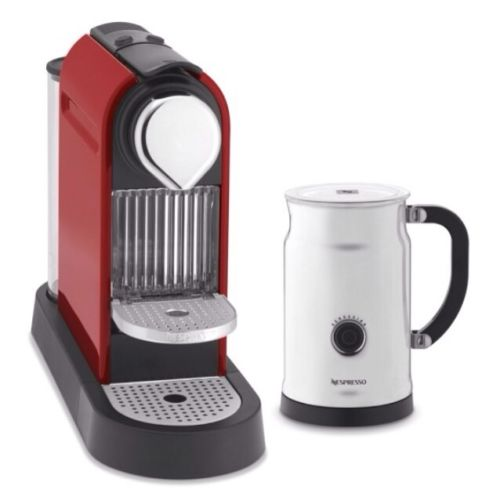
\includegraphics[scale=0.25]{images/ground_truth/4/image_1} & 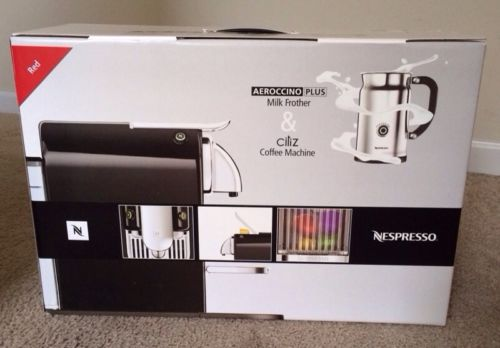
\includegraphics[scale=0.25]{images/ground_truth/4/image_2} & 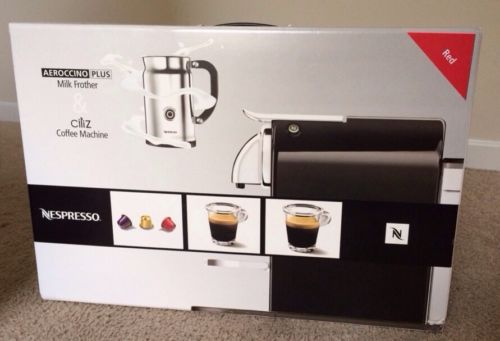
\includegraphics[scale=0.25]{images/ground_truth/4/image_3} \\
	\cline{2-4}
	\multirow{6}{*}{} & Title &  \multicolumn{2}{| p{10cm} |}{Nespresso Aeroccino Plus \& Citiz Coffee Machine {Red}} \\
	\cline{2-4}
	\multirow{6}{*}{} & Description &  \multicolumn{2}{| p{10cm} |}{Nespeesso Aeroccino Plus \& Citiz Coffee Machine Fully automatic brewing and milk frothing in two sleek, compact units. Works exclusively with Nespresso's premium coffee capsules, which are easy to order for delivery within two business days (for details, visit www.nespresso.com). Innovative Thermoblock technology with stainless-steel heating element guarantees precise temperature control. A 19-bar pressure pump ensures maximum extraction of flavor. Adjustable tray accommodates cups of various sizes (from small mug to travel cup). Removable water tank for easy refilling. Energy-save mode gradually reduces power if unit is left on. Includes Aeroccino Plus milk frother, which quickly heats milk for consistently perfect foam. Frother has two whisk attachments and an auto shutoff feature. Espresso maker: ABS plastic housing. 14 1/2" x 5" x 11" high. 34-fl.-oz.-cap. water tank. 10 lb. 1200W. Milk frother: Stainless-steel and plastic construction. 4" diam., 6-3/4" high. 8-oz. cap. 550W. This product is intended for use in the United States and Canada and is built to United States electrical standards. Posted with eBay Mobile} \\
	\cline{2-4}
	\multirow{6}{*}{} & Category &  \multicolumn{2}{| p{10cm} |}{Home \& Garden:Kitchen, Dining \& Bar:Small Kitchen Appliances:Coffee \& Tea Makers:Espresso Machines} \\
	\cline{2-4}
	\multirow{6}{*}{} & Condition &  \multicolumn{2}{| p{10cm} |}{New} \\
	\cline{2-4}
	\multirow{6}{*}{} & Price &  \multicolumn{2}{| p{10cm} |}{201.0} \\
	\hline \hline
	ID & Image 1 & Image 2 & Image 3 \\
	\hline
	\multirow{6}{*}{5} & 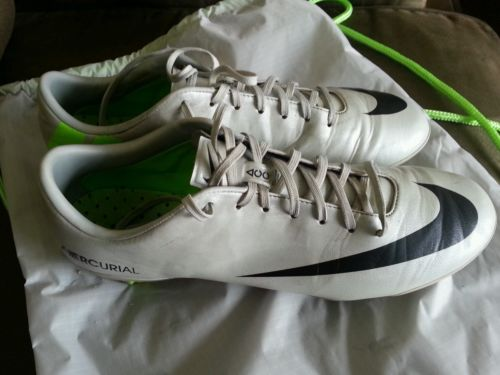
\includegraphics[scale=0.25]{images/ground_truth/5/image_1} & \includegraphics[scale=0.25]{images/ground_truth/5/image_2} & \includegraphics[scale=0.25]{images/ground_truth/5/image_3} \\
	\cline{2-4}
	\multirow{6}{*}{} & Title &  \multicolumn{2}{| p{10cm} |}{Nike Mercurial Vapor IX FG - Soccer Shoes Cleats - Metallic Platinum} \\
	\cline{2-4}
	\multirow{6}{*}{} & Description &  \multicolumn{2}{| p{10cm} |}{This is a pair of used Nike Vapor IX. They come with the string bag. In overall good condition with some signs of use. Clean and no smells. Mens size 7.5. Shipping is \$10.00 and includes tracking. I accept PayPal for payment.} \\
	\cline{2-4}
	\multirow{6}{*}{} & Category &  \multicolumn{2}{| p{10cm} |}{Sporting Goods:Team Sports:Soccer:Clothing, Shoes \& Accessories:Shoes \& Cleats:Men} \\
	\cline{2-4}
	\multirow{6}{*}{} & Condition &  \multicolumn{2}{| p{10cm} |}{Pre-owned} \\
	\cline{2-4}
	\multirow{6}{*}{} & Price &  \multicolumn{2}{| p{10cm} |}{76.99} \\
	\hline \hline
	ID & Image 1 & Image 2 & Image 3 \\
	\hline
	\multirow{6}{*}{6} & \includegraphics[scale=0.75]{images/ground_truth/6/image_1} & \includegraphics[scale=0.75]{images/ground_truth/6/image_2} & \includegraphics[scale=0.75]{images/ground_truth/6/image_3} \\
	\cline{2-4}
	\multirow{6}{*}{} & Title &  \multicolumn{2}{| p{10cm} |}{RARE Series 2 Palisades Resident Evil Code Veronica Alexia Action Figure} \\
	\cline{2-4}
	\multirow{6}{*}{} & Description &  \multicolumn{2}{| p{10cm} |}{This RARE and HARD TO FIND action figure will make and AWESOME collectable for any Resident Evil fan! This specific figure is part of the Resident Evil Code Veronica series. Alexia comes complete with Wings, Tail and Alternate Head to Transform into Alexia III and Logo Base. Great item for any RE fan!!! This item is still in its original packaging, unopened and unused. There is very slight wear around the cardboard edging from years of storage and a little adhesive residue on the plastic, most likely from a price sticker. Overall this item is in excellent condition!} \\
	\cline{2-4}
	\multirow{6}{*}{} & Category &  \multicolumn{2}{| p{10cm} |}{Toys \& Hobbies:Action Figures:TV, Movie \& Video Games} \\
	\cline{2-4}
	\multirow{6}{*}{} & Condition &  \multicolumn{2}{| p{10cm} |}{New} \\
	\cline{2-4}
	\multirow{6}{*}{} & Price &  \multicolumn{2}{| p{10cm} |}{90.0} \\
	\hline \hline
	ID & Image 1 & Image 2 & Image 3 \\
	\hline
	\multirow{6}{*}{7} & \includegraphics[scale=0.25]{images/ground_truth/7/image_1} & \includegraphics[scale=0.25]{images/ground_truth/7/image_2} & \includegraphics[scale=0.25]{images/ground_truth/7/image_3} \\
	\cline{2-4}
	\multirow{6}{*}{} & Title &  \multicolumn{2}{| p{10cm} |}{Black Coach purse leather GUC serial number H050-9247} \\
	\cline{2-4}
	\multirow{6}{*}{} & Description &  \multicolumn{2}{| p{10cm} |}{Pre-owned Black Coach hobo purse. GUC just because I did use it a couple of times. No stains,marks, or tears. Great condition!!!} \\
	\cline{2-4}
	\multirow{6}{*}{} & Category &  \multicolumn{2}{| p{10cm} |}{Clothing, Shoes \& Accessories:Women's Handbags \& Bags:Handbags \& Purses} \\
	\cline{2-4}
	\multirow{6}{*}{} & Condition &  \multicolumn{2}{| p{10cm} |}{Pre-owned} \\
	\cline{2-4}
	\multirow{6}{*}{} & Price &  \multicolumn{2}{| p{10cm} |}{35.0} \\
	\hline
\caption{Ground truth for pure crowdsourcing}
\end{longtable}

\section{Non-branded Item}
\begin{table}[h!]
	\begin{center}
	\begin{tabular}{| l | l | l |}
	\hline
	Image 1 & Image 2 & Image 3 \\
	\hline
	\includegraphics[scale=0.25]{images/ground_truth/8/image_1} & \includegraphics[scale=0.25]{images/ground_truth/8/image_2} & \includegraphics[scale=0.25]{images/ground_truth/8/image_3} \\
	\hline
	Title &  \multicolumn{2}{| p{10cm} |}{Saarinen Round Dining Table 47" White Laminate White Base KNOLL DWR} \\
	\hline
	Description &  \multicolumn{2}{| p{10cm} |}{Living Dining Outdoor Workspace Lighting Floor Accessories MidCentury Modern Saarinen Round Dining Table 47" (White Laminate/White Base) You are bidding on an AUTHENTIC Saarinen Round Dining Table, 47" in White Laminate with White base. Great condition, slight signs of handling. In a 1956 cover story in Time magazine, Eero Saarinen said he was designing a collection to "clear up the slum of legs in the U.S. home." Later that year, he completed his Pedestal Table and TulipTM Chair Collection (1956) and obliterated the "slum" by creating a cast aluminum base inspired by a drop of high-viscosity liquid. This table is manufactured by Knoll according to the original and exacting specifications of the designer. Made in Italy. Pedestal Tables come in a variety of table top materials (veneer, marble and laminate) and base colors (black, white and platinum).The base has an abrasion-resistant Rilsan finish.Each piece is stamped with the KnollStudio logo and Eero Saarinen's signature.Measurements: Assembled Table H 28.25" Diameter 47" Materials: Cast aluminum base with Rilsan finish; bevel-edged top in laminate Laminate: MDF with laminate.} \\
	\hline
	Category &  \multicolumn{2}{| p{10cm} |}{Home \& Garden:Furniture:Tables} \\
	\hline
	Condition &  \multicolumn{2}{| p{10cm} |}{Used} \\
	\hline
	Price &  \multicolumn{2}{| p{10cm} |}{1277.00} \\
	\hline
	\end{tabular}
	\end{center}
	\caption{Ground truth non-branded item}
\end{table}

\chapter{Machine Learning}
\section{Algorithms}
\section{Results}
\subsection{Significance}
\subsection{Classification}
\begin{figure}
\centering
\includegraphics[scale=0.55]{images/plots/machine_learning/mustang/true_pred_mustang.png}
\caption{Scatter plot true vs. prediction (Mustang)}
\label{crowdsourcing_desc_length}
\end{figure}
\begin{figure}
\centering
\includegraphics[scale=0.55]{images/plots/machine_learning/mustang/conf_mat_mustang.png}
\caption{Normalised confusion matrix (Mustang)}
\label{crowdsourcing_desc_length}
\end{figure}
\begin{figure}
\centering
\includegraphics[scale=0.55]{images/plots/machine_learning/playstation/true_pred_playstation.png}
\caption{Scatter plot true vs. prediction (Playstation)}
\label{crowdsourcing_desc_length}
\end{figure}
\begin{figure}
\centering
\includegraphics[scale=0.55]{images/plots/machine_learning/playstation/conf_mat_playstation.png}
\caption{Normalised confusion matrix (Playstation)}
\label{crowdsourcing_desc_length}
\end{figure}
\subsection{Regression}

\end{appendices}

\end{document}
